\documentclass{article}

\usepackage{arxiv}

\usepackage[utf8]{inputenc} % allow utf-8 input
\usepackage[T1]{fontenc}    % use 8-bit T1 fonts
\usepackage{hyperref}       % hyperlinks
\usepackage{url}            % simple URL typesetting
\usepackage{booktabs}       % professional-quality tables
\usepackage{amsfonts}       % blackboard math symbols
\usepackage{nicefrac}       % compact symbols for 1/2, etc.
\usepackage{microtype}      % microtypography
\usepackage{float}          % for [H] float placement
\usepackage{graphicx}
\usepackage{natbib}
\usepackage{doi}
\usepackage{tikz}
\usetikzlibrary{arrows.meta, patterns, calc}
\usepackage{amsmath}
\usepackage{amssymb}
\usepackage{bm}
\usepackage{xcolor}
\graphicspath{{./figures/}}

% Custom commands
\newcommand{\dd}{\mathrm{d}}
\newcommand{\Fr}{\mathrm{Fr}}
\newcommand{\We}{\mathrm{We}}
\newcommand{\Rey}{\mathrm{Re}}
\newcommand{\uu}{\mathbf{u}}
\newcommand{\ww}{\mathbf{w}}
\newcommand{\xx}{\mathbf{x}}
\newcommand{\bb}{\mathbf{b}}
\newcommand{\OO}{\mathcal{O}}

% Track-changes: content added in the latest revision is wrapped in
% blue via the \new{...} macro (for inline) or the \color{blue} / \color{black}
% switches (for multi-paragraph regions including display equations).
\newcommand{\new}[1]{{\color{blue}#1}}

\title{A monolithic solver for linearised Navier--Stokes free-surface dynamics via Helmholtz decomposition}

%\date{September 9, 1985}	% Here you can change the date presented in the paper title
%\date{} 					% Or removing it

\author{
  {Author~One}\thanks{Corresponding author.} \\
  {Department} \\
  {University} \\
  \texttt{author1@example.com} \\
  \And
  {Author~Two} \\
  {Department} \\
  {University} \\
  \texttt{author2@example.com} \\
}

\renewcommand{\shorttitle}{Monolithic LNS free-surface solver}

\hypersetup{
  pdftitle={A monolithic solver for linearised Navier--Stokes free-surface dynamics via Helmholtz decomposition},
  pdfsubject={physics.flu-dyn, math.NA},
  pdfauthor={Author One, Author Two},
  pdfkeywords={free surface dynamics, linearised Navier--Stokes, Helmholtz decomposition, monolithic solver, LU prefactorisation},
}

\begin{document}
\maketitle

%% ================================================================
%% ABSTRACT
%% ================================================================
\begin{abstract}
We present a numerical implementation of the linearised Navier--Stokes (LNS) free-surface model of \citet{GaleanoRiosEtAl2017}, which employs a Helmholtz decomposition of the velocity field into irrotational and vortical components.
The model solves the coupled system of Laplace's equation for the velocity potential, heat equations for the vortical fields, and surface evolution equations that incorporate gravity, surface tension, and viscous effects.
We implement both a sequential (operator-splitting) solver and a monolithic formulation in which all unknowns (the vortical components $w^3$ and $w^1$, the surface potential $\phi_s$, the bulk potential $\phi$, and the surface elevation $\eta$) are assembled into a single linear system $A\xx = \bb$.
Because the coefficient matrix $A$ is independent of the solution, it is factored once via sparse LU decomposition; each subsequent time step requires only $\OO(N)$ back-substitution.
We verify that the two formulations produce identical results to machine precision and demonstrate the computational advantage of the monolithic approach.
We further extend the same monolithic framework to fluid--body coupling by augmenting the unknown vector with the surface pressure, vertical position, and vertical velocity of a floating rigid body, yielding a fully implicit solver in which the body motion is determined self-consistently by Newton's second law driven by gravity and the integrated fluid pressure.
\end{abstract}

\keywords{Free surface dynamics \and linearised Navier--Stokes \and Helmholtz decomposition \and monolithic solver \and LU prefactorisation \and fluid--body coupling \and floating rigid body \and finite differences}

%% ================================================================
%% 1. INTRODUCTION
%% ================================================================
\section{Introduction}
\label{sec:intro}

The dynamics of viscous free-surface flows arise in numerous physical settings, from ocean wave propagation and droplet impact to the interaction of floating bodies with fluid baths.
While the full Navier--Stokes equations govern such flows, their nonlinearity and the need to track a moving free surface make direct numerical solution computationally expensive.
For problems where surface deflections are small relative to the fluid depth, a linearised approach can retain the essential physics---gravity, surface tension, and viscous dissipation---at greatly reduced cost.

\citet{GaleanoRiosEtAl2017} developed such a linearised Navier--Stokes (LNS) framework in the context of non-wetting sphere impact on a fluid bath and bouncing droplet dynamics.
The central idea is a Helmholtz decomposition of the velocity field $\uu = \nabla\phi + \ww$, which separates the flow into an irrotational component $\nabla\phi$ satisfying Laplace's equation in the bulk and a vortical component $\ww$ governed by the heat equation.
The two components are coupled through linearised boundary conditions at the free surface, which encode the kinematic condition (the surface moves with the fluid), the dynamic condition (normal stress balance including gravity, surface tension, and viscous effects), and a vorticity evolution equation.
At the bottom boundary, the non-slip condition $\uu = 0$ couples the vortical field to the potential field.

This framework was subsequently used by \citet{MilweskiEtAl2015} to study Faraday pilot-wave dynamics, by \citet{GaleanoRios2016} to investigate hydrodynamic pilot-wave resonance, and more recently by \citet{Barotta2025} in the context of macroscopic Brownian motion on chaotic fluid interfaces.
\citet{AgueroEtAl2022} applied the framework to the impact of a rigid sphere onto an elastic membrane, demonstrating its applicability to fluid--structure interaction problems.
The classical potential-flow foundations trace back to \citet{Lamb1932} and \citet{Batchelor1967}.

A common simplification employed in some implementations is the diagnostic relation $w^3 = (2/\Rey)\,\Delta_H\eta$ at the surface, derived by combining the kinematic and vorticity surface equations under the assumption that initial vorticity transients have decayed.
While this eliminates one unknown and is valid at high Reynolds numbers, it does not capture the full transient behaviour of the surface vorticity, and it precludes correct treatment of the non-slip bottom boundary condition for the vortical field.
In the present work, we solve the \emph{full} set of equations (2.15a--e) from \citet{GaleanoRiosEtAl2017}, evolving $w^3$ and $w^1$ as independent 2D fields via their respective heat equations, with proper boundary conditions at both the free surface and the solid bottom.

Our main contribution is a monolithic formulation of the full system.
In the standard sequential (operator-splitting) approach, each time step involves multiple sparse solves: the heat equations for $w^3$ and $w^1$, the implicit surface update for $\phi_s$, the Laplace equation for the bulk potential, and the kinematic update for $\eta$.
We show that the entire system can be assembled into a single block-structured linear system
\begin{equation*}
    A\,\xx^{n+1} = \bb(\xx^n),
\end{equation*}
where $\xx = [w^3,\, w^1,\, \phi_s,\, \phi_{\mathrm{bulk}},\, \eta]^\top$.
Because all equations are linear with constant coefficients, the matrix $A$ does not depend on the solution.
It is factored once via sparse LU decomposition at setup time, and each time step reduces to a single back-substitution at $\OO(N)$ cost.
We verify that the monolithic and sequential solvers produce identical results to machine precision, confirming the equivalence of the two formulations.

We then extend this framework to fluid--body coupling.
A flat-bottomed rigid body of finite width is placed on the free surface, and its motion is determined self-consistently by Newton's second law driven by gravity and the integrated fluid pressure.
Under the wetted region of the body, the standard free-surface boundary conditions are replaced by three constraints: a geometric constraint ($\eta$ matches the body position), a kinematic match (the vertical fluid velocity matches the body velocity), and horizontal no-slip at the body bottom.
The surface pressure $p_s$ acts as a Lagrange multiplier enforcing the kinematic match.
Augmenting the unknown vector by $p_s$ and the two body scalars $z_b, v_b$, the entire coupled system remains linear with constant coefficients, so it too is amenable to a one-time LU prefactorisation.
This fully implicit coupling avoids the added-mass instability that is known to afflict staggered fluid--body coupling schemes, particularly for light bodies.

The remainder of this paper is organised as follows.
Section~\ref{sec:formulation} presents the mathematical model: the Helmholtz decomposition, the governing equations in the bulk and at the boundaries, the non-dimensionalisation, and the extension to fluid--body coupling for a floating rigid body.
Section~\ref{sec:numerical} describes the numerical methods: finite difference discretisation, the sequential time-stepping algorithm, the monolithic system assembly for the pure fluid problem, and the augmented monolithic system for the coupled fluid--body problem.
Section~\ref{sec:results} presents numerical results.
% TODO: Expand outline once results are finalised.

%% ================================================================
%% 2. MATHEMATICAL MODEL
%% ================================================================
\section{Mathematical model}
\label{sec:formulation}

\subsection{Physical setup}
\label{sec:setup}

We consider a two-dimensional domain with horizontal coordinate $x' \in [0, L']$ and vertical coordinate $z'$, where $z' = 0$ is at the mean free surface and $z' = -D'$ is at the solid bottom.
The fluid has density $\rho$, kinematic viscosity $\nu$, and surface tension coefficient $\sigma$.
The free surface is located at $z' = \eta'(x', t')$, where $\eta'$ is the surface elevation.
Primes denote dimensional variables.

We assume that surface deflections are small relative to the depth ($|\eta'| \ll D'$), so that the free-surface boundary conditions can be linearised about $z' = 0$.
Horizontal boundary conditions are periodic: $\eta'(0, t') = \eta'(L', t')$, and similarly for all other fields.

\subsection{Helmholtz decomposition}
\color{blue}
\label{sec:helmholtz}

Following \citet{GaleanoRiosEtAl2017}, the velocity field is decomposed as
\begin{equation}
    \uu = \nabla\phi + \ww, \label{eq:helmholtz}
\end{equation}
where $\phi(x', z', t')$ is a scalar potential and $\ww(x', z', t') = (w^{\prime 1}, w^{\prime 2}, w^{\prime 3})$ is a vector field carrying the vortical (rotational) part of the flow.
In the present two-dimensional setting, the out-of-plane component vanishes by symmetry, $w^{\prime 2} = 0$, and we write $\ww = (w^{\prime 1}, w^{\prime 3})$, where $w^{\prime 1}$ and $w^{\prime 3}$ are the horizontal and vertical components of the vortical field, respectively.

The decomposition~\eqref{eq:helmholtz} is not unique: for any scalar $\psi$ satisfying $\Delta\psi = 0$, one can add $\nabla\psi$ to $\nabla\phi$ and subtract it from $\ww$ without altering $\uu$.
We remove this ambiguity by demanding that the potential carry the entire irrotational part of $\uu$, equivalently that $\ww$ be solenoidal:
\begin{equation}
    \nabla \cdot \ww = 0. \label{eq:w_solenoidal}
\end{equation}
Taking the divergence of~\eqref{eq:helmholtz} and using both~\eqref{eq:w_solenoidal} and the incompressibility of the fluid $\nabla \cdot \uu = 0$, we have
\begin{equation}
    0 \;=\; \nabla \cdot \uu \;=\; \nabla \cdot (\nabla\phi) + \nabla \cdot \ww \;=\; \Delta\phi, \label{eq:laplace_derivation}
\end{equation}
i.e.\ the potential is harmonic in the bulk.
Moreover, since $\nabla \times \nabla\phi = \bm{0}$ identically, the entire vorticity of the flow is carried by the vortical part,
\begin{equation}
    \nabla \times \uu \;=\; \nabla \times \ww. \label{eq:vorticity_in_w}
\end{equation}

To derive the bulk equation governing $\ww$, we start from the linearised Navier--Stokes equation
\begin{equation}
    \partial_{t'}\uu \;=\; -\frac{1}{\rho}\,\nabla p' + \nu\,\Delta\uu - g\,\hat{\bm{z}}, \label{eq:LNS_bulk_dim}
\end{equation}
where $p'$ is the dimensional pressure and $\hat{\bm{z}}$ is the unit vector pointing opposite to gravity.
The nonlinear convective term $(\uu\cdot\nabla)\uu$ has been dropped on the basis that surface deflections, and therefore the fluid velocities they induce, are small compared with the characteristic scales of the problem (see Section~\ref{sec:setup}).
Substituting~\eqref{eq:helmholtz} into~\eqref{eq:LNS_bulk_dim} and using $\Delta\phi = 0$ to suppress the diffusive contribution from the potential part, we obtain
\begin{equation}
    \nabla(\partial_{t'}\phi) + \partial_{t'}\ww \;=\; -\frac{1}{\rho}\,\nabla p' + \nu\,\Delta\ww - g\,\hat{\bm{z}}. \label{eq:LNS_decomposed}
\end{equation}
The right-hand side of~\eqref{eq:LNS_decomposed} separates into a gradient part---which represents the irrotational dynamics and absorbs both pressure and gravity---and a non-gradient part, which represents the vortical dynamics.
Matching the gradient and non-gradient parts of~\eqref{eq:LNS_decomposed} separately, we identify
\begin{align}
    \partial_{t'}\phi \;&=\; -\frac{p'}{\rho} - g z', \label{eq:bernoulli_bulk} \\
    \partial_{t'}\ww \;&=\; \nu\,\Delta\ww, \label{eq:heat_dim_derivation}
\end{align}
where any spatially constant integration term has been absorbed into the gauge freedom of $\phi$.
Equation~\eqref{eq:bernoulli_bulk} is the linearised Bernoulli relation valid throughout the bulk; it determines how the pressure responds to the time rate of change of the potential and to the hydrostatic head.
\color{black}
Equation~\eqref{eq:heat_dim_derivation} is the heat equation: each Cartesian component of the vortical field diffuses with kinematic viscosity~$\nu$ and, crucially, does not self-advect---this last property being a direct consequence of the linearisation.

The appeal of the decomposition is now twofold.
First, the irrotational part $\nabla\phi$ satisfies an elliptic, time-independent equation in the bulk, so it can be solved by standard sparse linear algebra once boundary data are specified.
Second, the vortical part $\ww$ is governed by parabolic equations whose sources are concentrated at the boundaries, so that for moderate-to-high Reynolds numbers the bulk flow is dominated by the potential while the vortical component is confined to thin diffusive layers near the free surface and the solid bottom.
The two fields are uncoupled in the bulk; their interaction takes place \emph{exclusively} through the boundary conditions at $z' = 0$ and $z' = -D'$, derived in the next section.
\color{blue}

\subsection{Governing equations}
\label{sec:governing}

\subsubsection{Bulk equations}

In the interior of the fluid domain ($-D' < z' < 0$), the potential satisfies Laplace's equation and each vortical component satisfies the heat equation:
\begin{align}
    \Delta\phi \;&=\; 0, \label{eq:laplace} \\
    \partial_{t'} w^{\prime i} \;&=\; \nu\, \Delta w^{\prime i}, \qquad i = 1, 3. \label{eq:heat}
\end{align}
\color{black}
Equation~\eqref{eq:laplace} was derived in Section~\ref{sec:helmholtz} (cf.~\eqref{eq:laplace_derivation}) from the incompressibility constraint and the solenoidal property~\eqref{eq:w_solenoidal} of $\ww$; it is time-independent, so the potential field adjusts instantaneously to whatever boundary data are specified at the surface and at the bottom.
Equation~\eqref{eq:heat}, derived as~\eqref{eq:heat_dim_derivation}, follows directly from the linearised Navier--Stokes equation~\eqref{eq:LNS_bulk_dim} after the Helmholtz decomposition is substituted and the gradient and rotational parts are separated.
\color{blue}

The bulk equations~\eqref{eq:laplace}--\eqref{eq:heat} are decoupled: $\phi$ satisfies an elliptic equation and the components of $\ww$ each satisfy a parabolic equation with no cross-coupling.
All coupling between potential and vortical degrees of freedom therefore occurs through the boundary conditions, which we derive below.
We also note that the pressure does not appear as an independent unknown: it has been absorbed into the Bernoulli relation~\eqref{eq:bernoulli_bulk}, which determines $p'$ algebraically in terms of $\phi$ and $z'$.

\subsubsection{Free-surface boundary conditions (\texorpdfstring{$z' = 0$}{z' = 0})}
\label{sec:bc_free_surface}

Under the small-amplitude assumption $|\eta'| \ll D'$, the free-surface boundary conditions can be evaluated at the mean surface level $z' = 0$ rather than at the actual deformed surface $z' = \eta'$.
This linearisation is the essential simplification that turns an otherwise nonlinear moving-boundary problem into a linear system on a fixed domain.
Three physical requirements must be imposed at the free surface: a \emph{kinematic} condition stating that the surface moves with the fluid, a \emph{dynamic} condition balancing normal stresses at the interface, and a \emph{vorticity} condition derived from the evolution of the surface vortical component.
In addition, a \emph{stress-free} condition on the horizontal vortical component $w^{\prime 1}$ closes the system.
We derive each of these conditions in turn (cf.\ \citealt{GaleanoRiosEtAl2017}, equations~2.15c--e and~2.11a).

\paragraph{Kinematic condition (KBC).}
A material particle on the free surface must remain on the free surface.
Writing the surface implicitly as $F(x', z', t') := z' - \eta'(x', t') = 0$, this Lagrangian condition reads
\begin{equation}
    \frac{\mathrm{D} F}{\mathrm{D} t'} \;=\; \partial_{t'} F + (\uu \cdot \nabla) F \;=\; 0 \qquad \text{on } z' = \eta'(x', t'), \label{eq:KBC_material}
\end{equation}
which, on substituting $F = z' - \eta'$, gives
\begin{equation}
    -\partial_{t'}\eta' - u'_{x'}\,\partial_{x'}\eta' + u'_{z'} \;=\; 0 \qquad \text{on } z' = \eta'. \label{eq:KBC_nonlinear}
\end{equation}
Linearising around the rest state ($\eta', u'_{x'}, u'_{z'}$ all small) drops the product $u'_{x'} \partial_{x'}\eta'$ and evaluates the remaining quantities at $z' = 0$:
\begin{equation}
    \partial_{t'}\eta' \;=\; u'_{z'}\big|_{z' = 0} \;=\; \partial_{z'}\phi' + w^{\prime 3} \qquad \text{at } z' = 0, \label{eq:surf_kin}
\end{equation}
where the second equality uses the Helmholtz decomposition~\eqref{eq:helmholtz}.
Equation~\eqref{eq:surf_kin} is the kinematic boundary condition (henceforth KBC).

\paragraph{Dynamic condition (DBC).}
The dynamic boundary condition expresses the balance of stresses across the free surface.
For a Newtonian fluid the stress tensor takes the form
\begin{equation}
    \bm{\sigma} \;=\; -p'\,\bm{I} + \mu\,\big[\nabla\uu + (\nabla\uu)^{\top}\big], \label{eq:stress_tensor}
\end{equation}
where $\mu = \rho\nu$ is the dynamic viscosity.
At the free surface, jumping from the fluid side to the ambient side, the normal-stress balance equates the fluid's normal traction to the atmospheric pressure plus the capillary contribution $-\sigma\kappa[\eta']$,
\begin{equation}
    \bm{n} \cdot \bm{\sigma} \cdot \bm{n} \;=\; -p'_s - \sigma\,\kappa[\eta'], \label{eq:normal_stress_balance}
\end{equation}
where $\bm{n}$ is the outward unit normal, $p'_s(x', t')$ denotes any externally applied surface pressure (zero for an uncovered free surface), and $\kappa[\eta']$ is the mean curvature of the interface.
For small slopes the linearised normal is $\bm{n} \approx (-\partial_{x'}\eta',\, 1)$, the leading-order normal becomes $\bm{n} \approx \hat{\bm{z}}$, and the curvature reduces to $\kappa[\eta'] \approx -\partial_{x'x'}\eta'$ (with our sign convention that a crest has $\partial_{x'x'}\eta' < 0$).
The leading-order normal-stress component is therefore
\begin{equation}
    \bm{n}\cdot\bm{\sigma}\cdot\bm{n}\big|_{z' = 0} \;=\; -p'\big|_{z' = 0} + 2\mu\,\partial_{z'}u'_{z'}\big|_{z' = 0}. \label{eq:normal_stress_linearised}
\end{equation}
We evaluate $p'$ at the (deformed) surface using the linearised Bernoulli relation~\eqref{eq:bernoulli_bulk} at $z' = \eta'$ and a Taylor expansion about $z' = 0$,
\begin{equation}
    p'(x', \eta', t') \;\approx\; p'(x', 0, t') + \eta'\,\partial_{z'}p'(x', 0, t') \;\approx\; -\rho\,\partial_{t'}\phi'_s - \rho g\,\eta', \label{eq:bernoulli_at_surface}
\end{equation}
where $\phi'_s(x', t') := \phi'(x', 0, t')$ is the surface potential and the hydrostatic part $-\rho g\,\eta'$ comes from the Taylor expansion (since at leading order $\partial_{z'}p' = -\rho g$).
Substituting~\eqref{eq:bernoulli_at_surface} together with $u'_{z'} = \partial_{z'}\phi' + w^{\prime 3}$ into the normal-stress balance~\eqref{eq:normal_stress_balance}, we obtain
\begin{equation}
    \rho\,\partial_{t'}\phi'_s + \rho g\,\eta' + 2\mu\,\big(\partial_{z'z'}\phi' + \partial_{z'} w^{\prime 3}\big) \;=\; -p'_s + \sigma\,\partial_{x'x'}\eta'. \label{eq:dyn_intermediate}
\end{equation}
Dividing through by~$\rho$, using $\nu = \mu/\rho$, and finally invoking $\partial_{z'z'}\phi' = -\partial_{x'x'}\phi'_s$ (which is the Laplace equation~\eqref{eq:laplace} restricted to $z' = 0$), we arrive at
\begin{equation}
    \partial_{t'}\phi'_s \;=\; -g\eta' + \frac{\sigma}{\rho}\,\partial_{x'x'}\eta' + 2\nu\,\partial_{x'x'}\phi'_s - 2\nu\,\partial_{z'} w^{\prime 3} - \frac{p'_s}{\rho}. \label{eq:surf_dyn}
\end{equation}
Equation~\eqref{eq:surf_dyn} is the dynamic boundary condition (henceforth DBC).
The four right-hand-side terms admit a transparent physical interpretation:
the first ($-g\eta'$) is the hydrostatic restoring force that drives gravity waves;
the second ($(\sigma/\rho)\,\partial_{x'x'}\eta'$) is the capillary restoring force from surface tension;
the third ($2\nu\,\partial_{x'x'}\phi'_s$) is the tangential viscous stress associated with the horizontal curvature of the surface potential;
and the fourth ($-2\nu\,\partial_{z'} w^{\prime 3}$) couples the surface potential to the vortical field through the vertical gradient of $w^{\prime 3}$.
The last term is essential: it is the reason the surface potential and the vortical component do not decouple, even under the linearisation.

\paragraph{Vorticity evolution at the surface (VEQ).}
A surface evolution equation for $w^{\prime 3}$ can be obtained by combining the kinematic condition~\eqref{eq:surf_kin} with the tangential stress-free condition (DBC$_{\mathrm{tang}}$, derived in Section~\ref{sec:stress_free_w1} below).
\color{black}
Differentiating~\eqref{eq:surf_kin} twice in $x'$ and using the standard identity $\partial_{t'} \partial_{x'x'}\eta' = \partial_{x'x'}\partial_{t'}\eta'$, one finds (cf.~\citealt{GaleanoRiosEtAl2017}, derivation of eq.~2.15e) that the surface value of $w^{\prime 3}$ obeys
\begin{equation}
\color{blue}
    \partial_{t'} w^{\prime 3} \;=\; 2\nu\, \partial_{x'x'}\!\left(\partial_{z'}\phi' + w^{\prime 3}\right) \qquad \text{at } z' = 0. \label{eq:surf_vort}
\end{equation}
We refer to~\eqref{eq:surf_vort} as the surface vorticity equation (VEQ).
An equivalent derivation, more directly tied to the bulk physics, is given in Section~\ref{sec:inclusive_treatment}: there we show that the same relation~\eqref{eq:surf_vort} follows from imposing the bulk heat equation~\eqref{eq:heat} inclusively at $z' = 0$ together with the stress-free condition for $w^{\prime 1}$.

\subsubsection{Bottom boundary condition (\texorpdfstring{$z' = -D'$}{z' = -D'})}
\label{sec:bc_bottom}

The fluid is bounded below by a rigid, impermeable, stationary wall at $z' = -D'$, on which both components of the velocity must vanish.
We therefore impose the non-slip condition $\uu = \bm{0}$ at $z' = -D'$.
Writing this component-wise using the Helmholtz decomposition~\eqref{eq:helmholtz},
\begin{align}
    u'_{x'}\big|_{z'=-D'} \;&=\; \partial_{x'}\phi' + w^{\prime 1} \;=\; 0, \label{eq:bot_x_velocity} \\
    u'_{z'}\big|_{z'=-D'} \;&=\; \partial_{z'}\phi' + w^{\prime 3} \;=\; 0, \label{eq:bot_z_velocity}
\end{align}
which rearrange to
\color{black}
\begin{align}
\color{blue}
    w^{\prime 3} \;&=\; -\partial_{z'}\phi' \qquad \text{at } z' = -D', \label{eq:bc_bot_w3} \\
    w^{\prime 1} \;&=\; -\partial_{x'}\phi' \qquad \text{at } z' = -D'. \label{eq:bc_bot_w1}
\end{align}
Equations~\eqref{eq:bc_bot_w3}--\eqref{eq:bc_bot_w1} express the bottom boundary condition as a Dirichlet-type coupling between the vortical and potential fields: at the wall, $\ww$ is locked to $-\nabla\phi'$ so that their sum vanishes.
Physically, this requirement embodies the no-penetration condition (vertical velocity zero) and the no-slip condition (horizontal velocity zero) at the rigid bottom, simultaneously.

\subsubsection{Stress-free (tangential) condition at the surface}
\label{sec:stress_free_w1}

The free surface is by assumption an interface with an inviscid gas of negligible mass; consequently the tangential viscous stress must vanish there.
For the linearised, nearly flat surface the tangent direction is $\bm{t} \approx \hat{\bm{x}}$ and the normal is $\bm{n} \approx \hat{\bm{z}}$, so the tangential stress component reduces to the $(x', z')$ component of the symmetric rate-of-strain tensor times $2\mu$:
\begin{equation}
    \bm{t}\cdot\bm{\sigma}\cdot\bm{n}\big|_{z'=0} \;=\; \mu\,\big(\partial_{z'}u'_{x'} + \partial_{x'}u'_{z'}\big)\big|_{z'=0} \;=\; 0. \label{eq:tang_stress_zero}
\end{equation}
Now using the Helmholtz decomposition~\eqref{eq:helmholtz} to write $u'_{x'} = \partial_{x'}\phi' + w^{\prime 1}$ and $u'_{z'} = \partial_{z'}\phi' + w^{\prime 3}$, each velocity gradient in~\eqref{eq:tang_stress_zero} produces \emph{two} contributions---one from the potential and one from the vortical part:
\begin{align}
    \partial_{z'}u'_{x'} \;&=\; \partial_{x'z'}\phi' + \partial_{z'} w^{\prime 1}, \label{eq:dz_ux} \\
    \partial_{x'}u'_{z'} \;&=\; \partial_{x'z'}\phi' + \partial_{x'} w^{\prime 3}. \label{eq:dx_uz}
\end{align}
Adding~\eqref{eq:dz_ux} and~\eqref{eq:dx_uz} and demanding that their sum vanish yields the tangential stress-free condition (DBC$_{\mathrm{tang}}$)
\begin{equation}
    2\,\partial_{x'z'}\phi' + \partial_{z'} w^{\prime 1} + \partial_{x'} w^{\prime 3} \;=\; 0 \qquad \text{at } z' = 0, \label{eq:bc_surf_w1}
\end{equation}
or, equivalently,
\begin{equation}
    \partial_{z'} w^{\prime 1} \;=\; -\big(2\,\partial_{x'z'}\phi' + \partial_{x'} w^{\prime 3}\big) \qquad \text{at } z' = 0. \label{eq:bc_surf_w1_explicit}
\end{equation}
The \emph{factor of two} in front of $\partial_{x'z'}\phi'$ is the central feature of~\eqref{eq:bc_surf_w1}.
It arises because the mixed derivative $\partial_{x'z'}\phi'$ appears once as $\partial_{z'}(\partial_{x'}\phi')$ in~\eqref{eq:dz_ux} and once as $\partial_{x'}(\partial_{z'}\phi')$ in~\eqref{eq:dx_uz}.
An earlier draft (v2) of the present implementation inadvertently retained a single factor of $\partial_{x'z'}\phi'$ in~\eqref{eq:bc_surf_w1} (cf.\ \citealt{GaleanoRiosEtAl2017}, equation~2.11a), which slightly over-estimated the viscous coupling between the potential and the surface vortical field; that error is corrected in the present (v3) formulation.

\subsubsection{Inclusive treatment of the bulk heat equation at the surface}
\label{sec:inclusive_treatment}

In the formulation presented so far, the surface vortical component $w^{\prime 3}$ is governed by the dedicated surface vorticity equation~\eqref{eq:surf_vort}, while the bulk value of $w^{\prime 3}$ at $z' < 0$ is governed by the heat equation~\eqref{eq:heat}.
An equivalent and---numerically---more convenient point of view is to impose the bulk heat equation~\eqref{eq:heat} \emph{inclusively} up to and including the surface $z' = 0$, with the second vertical derivative interpreted via a one-sided stencil that incorporates the surface boundary information.

To see the equivalence, we differentiate the solenoidal property~\eqref{eq:w_solenoidal} in the form $\partial_{z'} w^{\prime 3} = -\partial_{x'} w^{\prime 1}$ once more in $z'$ to obtain
\begin{equation}
    \partial_{z'z'} w^{\prime 3} \;=\; -\partial_{x'z'} w^{\prime 1}. \label{eq:dzz_w3_via_continuity}
\end{equation}
We then differentiate the tangential stress-free condition~\eqref{eq:bc_surf_w1} in $x'$,
\begin{equation}
    \partial_{x'z'} w^{\prime 1} \;=\; -\big(2\,\partial_{x'x'z'}\phi' + \partial_{x'x'} w^{\prime 3}\big), \label{eq:dxz_w1_from_DBC_tang}
\end{equation}
and substitute~\eqref{eq:dxz_w1_from_DBC_tang} into~\eqref{eq:dzz_w3_via_continuity} to obtain
\begin{equation}
    \partial_{z'z'} w^{\prime 3}\big|_{z'=0} \;=\; 2\,\partial_{x'x'z'}\phi' + \partial_{x'x'} w^{\prime 3}. \label{eq:dzz_w3_at_surface}
\end{equation}
The bulk heat equation~\eqref{eq:heat} evaluated at $z' = 0$ then reads
\begin{equation}
    \partial_{t'} w^{\prime 3} \;=\; \nu\,\big(\partial_{x'x'} w^{\prime 3} + \partial_{z'z'} w^{\prime 3}\big)\big|_{z'=0} \;=\; \nu\,\big(2\,\partial_{x'x'} w^{\prime 3} + 2\,\partial_{x'x'z'}\phi'\big), \label{eq:heat_at_surface_subst}
\end{equation}
which simplifies to
\color{black}
\begin{equation}
\color{blue}
    \partial_{t'} w^{\prime 3} \;=\; 2\nu\,\partial_{x'x'}\!\big(w^{\prime 3} + \partial_{z'}\phi'\big) \qquad \text{at } z' = 0, \label{eq:surf_vort_recovered}
\end{equation}
which is precisely the surface vorticity equation~\eqref{eq:surf_vort}.
This derivation shows that, provided the bulk heat equation~\eqref{eq:heat} is applied inclusively up to $z' = 0$ (with $\partial_{z'z'} w^{\prime 3}$ interpreted via the stress-free constraint), no separate evolution equation for $w^{\prime 3}|_{z'=0}$ is needed: it is automatically implied.
In our numerical scheme (Section~\ref{sec:numerical}), this observation underwrites a uniform discretisation of the bulk heat operator throughout $-D' \le z' \le 0$, with the surface row of the resulting matrix containing one-sided differences that respect~\eqref{eq:bc_surf_w1}.

\paragraph{Remark on the high-Reynolds diagnostic relation (GR2017, eq.~2.17).}
Combining the kinematic condition~\eqref{eq:surf_kin} and the surface vorticity equation~\eqref{eq:surf_vort} and integrating in time, one obtains, in the limit where all initial surface-vorticity transients have decayed, the diagnostic relation
\begin{equation}
    w^{\prime 3} \;=\; 2\nu\, \Delta_H' \eta' \qquad \text{at } z' = 0,
    \label{eq:w3_diagnostic_remark}
\color{black}
\end{equation}
which is widely used in the high-Reynolds-number droplet/bouncing literature \citep{GaleanoRiosEtAl2017}.
\color{blue}
This simplification is appealing because it eliminates one partial differential equation from the surface system; however, its validity rests on two conditions that are not always met: first, the initial state must have no residual surface vorticity, and second, the Reynolds number must be large enough that transient vortical dynamics are negligible on the timescale of interest.
Moreover, if the diagnostic relation is used, the vortical field loses its own degree of freedom at the surface, and the non-slip bottom boundary condition~\eqref{eq:bc_bot_w3}--\eqref{eq:bc_bot_w1} can no longer be imposed independently of the potential.
In the present implementation we therefore retain equation~\eqref{eq:surf_vort}---or, equivalently, the inclusive treatment of Section~\ref{sec:inclusive_treatment}---as an independent evolution of the surface $w^{\prime 3}$, solve the bulk heat equations~\eqref{eq:heat} for $w^{\prime 1}$ and $w^{\prime 3}$ throughout the domain, and impose the full non-slip bottom condition separately.
This design admits a wider range of initial conditions, faithfully captures the short-time transient behaviour at the surface, and permits the surface- and bottom-boundary layers to be resolved independently.

\color{black}
\subsection{Summary of the model}
\label{sec:model_summary}

For ease of reference and to make explicit the piecewise structure of the surface conditions induced by the floating body, we collect the full set of governing equations in their dimensionless form below.
The free-surface region is $\{z = 0,\; x > L\}$, where $L = x_c - a$ denotes the right edge of the body's footprint (and the domain has been restricted to $x \in [0, D]$ exploiting the reflection symmetry about $x = x_c$), while the wetted region is $\{z = 0,\; x \leq L\}$.
We use $h(t)$ for the body's vertical position and $v(t)$ for its vertical velocity; the contact half-width is denoted by $c$ in the summary so that $\eta = h - c$ corresponds to the linearised geometric constraint $\eta = z_b$ at the body's bottom (cf.~\eqref{eq:body_eta_constraint}).
\begin{subequations}
\begin{align}
    \Delta \phi &=0,& \qquad -H<z<0,t>0;\\
    w^1_t &= \frac{1}{\Rey}\Delta w^1,& \qquad -H<z<0,t>0;\\
    w^3_t &= \frac{1}{\Rey}\Delta w^3,& \qquad -H<z<0,t>0;\\
    \eta_t &= \phi_z+w^3,& \qquad z=0,t>0;\\
    \phi_t &= -\frac{1}{\Fr}\eta+\frac{1}{\We}\kappa\left[\eta\right]+\frac{2}{\Rey}\Delta_H\phi-\frac{2}{\Rey}w^3_z,& \qquad z=0, x>L,t>0;\\
    \color{blue}\eta &\color{blue}= h-c,&\color{blue} \qquad z=0, x\leq L,t>0;\color{black}\\
    2\phi_{xz}+w^1_z+w^3_x&=0,&z=0,x>L,t>0;\\
     \phi_x &= -w^1,& \qquad z= 0, x\leq L,t>0; \\
    \phi_x &= -w^1,& \qquad z= -H,t>0; \\
    \phi_z &= -w^3,& \qquad z= -H,t>0; \\
    h_t &= v,& \qquad t>0;\\
    v_t &= -\frac{1}{\Fr} + {\color{blue}2\sigma \sin(\arctan(\eta_x))} + \frac{1}{Ma}\int_0^L{\left[-\phi_t-\frac{1}{\Fr}\eta-\frac{2}{\Rey}\left(\phi_z+w^3\right)_z\right]},& \qquad t>0.
\end{align}
subject to all odd-order derivatives with respect to $x$ of $\eta$, $\phi$, $w^1$ and $w^3$ being equals to $0$ at $x=0$ and $x=D$.
\end{subequations}

\color{blue}
\noindent
\fbox{\begin{minipage}{0.97\linewidth}\small
\textbf{Equivalence with the Lagrange-multiplier form.}\;
Equation~(2.32) above is the body Newton's law in \emph{explicit-traction} form: the fluid traction on the bottom of the body is written out directly as $\tau_z = -\phi_t - \eta/\Fr - (2/\Rey)(\phi_z + w^3)_z$, integrated over the wetted region, and the lateral surface tension at the two contact lines contributes the separate term $2\sigma\sin(\arctan(\eta_x))$.
The identical body trajectory is obtained from the \emph{Lagrange-multiplier} form
\begin{equation*}
    M\,v_t \;=\; -\frac{M}{\Fr} \;+\; \int_{\mathcal{B}} p_s(x,t)\,\mathrm{d} x,
\end{equation*}
in which $p_s$ on the wetted region is left as an unknown that enforces the kinematic match $\phi_z + w^3 = v$ at every point under the body, and the surface dynamic condition~(2.24) still holds inside~$\mathcal{B}$.
Substituting that dynamic condition algebraically for $p_s$ recovers~(2.32) line by line, the contact-line term emerging from $\int_{\mathcal{B}}(1/\We)\,\partial_{xx}\eta\,\mathrm{d} x = (1/\We)[\partial_x\eta]_{x_c-a}^{x_c+a}$; the full derivation is given in Section~\ref{sec:explicit_traction}.
The two forms are mathematically equivalent; the Lagrange-multiplier form is preferred numerically because it yields a sparser block structure (Section~\ref{sec:augmented_monolithic}).
\end{minipage}}
\color{black}



\subsection{Non-dimensionalisation}
\label{sec:nondim}

We non-dimensionalise using a characteristic length $L_c$ and velocity $V_c = L_c / T_c$:
\begin{equation}
    x = \frac{x'}{L_c}, \quad z = \frac{z'}{L_c}, \quad t = \frac{t'}{T_c}, \quad \eta = \frac{\eta'}{L_c}, \quad \phi = \frac{\phi'}{V_c L_c}.
    \label{eq:nondim}
\end{equation}
This introduces the dimensionless numbers
\begin{equation}
    \Fr = \frac{V_c^2}{g L_c}, \qquad
    \We = \frac{\rho\, V_c^2 L_c}{\sigma}, \qquad
    \Rey = \frac{V_c L_c}{\nu}.
    \label{eq:dimless}
\end{equation}
The Froude number $\Fr$ measures the ratio of inertia to gravity; for $\Fr \gg 1$ inertia dominates and gravity waves are weakly restored, while for $\Fr \ll 1$ gravity strongly constrains surface motion.
The Weber number $\We$ measures the ratio of inertia to capillarity; large $\We$ corresponds to a weakly capillary regime in which surface tension is unimportant at the scale $L_c$, whereas small $\We$ puts surface tension in the leading role.
The Reynolds number $\Rey$ measures the ratio of inertia to viscous diffusion; free-surface wave problems of interest typically have $\Rey$ ranging from $\OO(10^2)$ for millimetric droplets to $\OO(10^5)$--$\OO(10^6)$ for centimetric or larger bodies in water.
These three groups are sufficient to characterise the dynamics of the pure fluid problem; an additional parameter $M$, introduced in Section~\ref{sec:floating_body}, governs the coupled fluid--body dynamics.

The dimensionless governing equations become:

\paragraph{Bulk:}
\begin{align}
    \Delta\phi &= 0, \quad z \leq 0, \label{eq:nd_laplace} \\
    \partial_t w^i &= \frac{1}{\Rey}\,\Delta w^i, \quad z \leq 0, \quad i = 1,3. \label{eq:nd_heat}
\end{align}

\paragraph{Free surface ($z = 0$):}
\begin{align}
    \partial_t \eta &= \partial_z \phi + w^3, \label{eq:nd_kin} \\
    \partial_t \phi_s &= -\frac{1}{\Fr}\,\eta + \frac{1}{\We}\,\partial_{xx}\eta + \frac{2}{\Rey}\,\partial_{xx} \phi_s - \frac{2}{\Rey}\,\partial_z w^3, \label{eq:nd_dyn} \\
    \partial_t w^3 &= \frac{2}{\Rey}\,\partial_{xx}\!\left(\partial_z\phi + w^3\right). \label{eq:nd_vort}
\end{align}

\paragraph{Bottom ($z = -D$):}
\begin{align}
    w^3 &= -\partial_z\phi, \label{eq:nd_bot_w3} \\
    w^1 &= -\partial_x\phi. \label{eq:nd_bot_w1}
\end{align}

\paragraph{Surface stress-free for $w^1$:}
\begin{equation}
    \partial_z w^1 = -(\partial_{xz}\phi + \partial_x w^3) \quad \text{at } z = 0. \label{eq:nd_surf_w1}
\end{equation}

\subsection{Extension to a floating rigid body}
\label{sec:floating_body}

The LNS framework extends naturally to the case of a rigid body floating on the fluid surface.
We consider a flat-bottomed rectangular body of half-width $a$ and mass per unit length $m$, centred at $x = x_c$, whose bottom lies at dimensional vertical position $z'_b(t')$ with vertical velocity $v'_b(t') = \mathrm{d} z'_b / \mathrm{d} t'$.
The geometric setup is illustrated in Figure~\ref{fig:schematic_2D}.

\color{blue}
\begin{figure}[H]
\centering
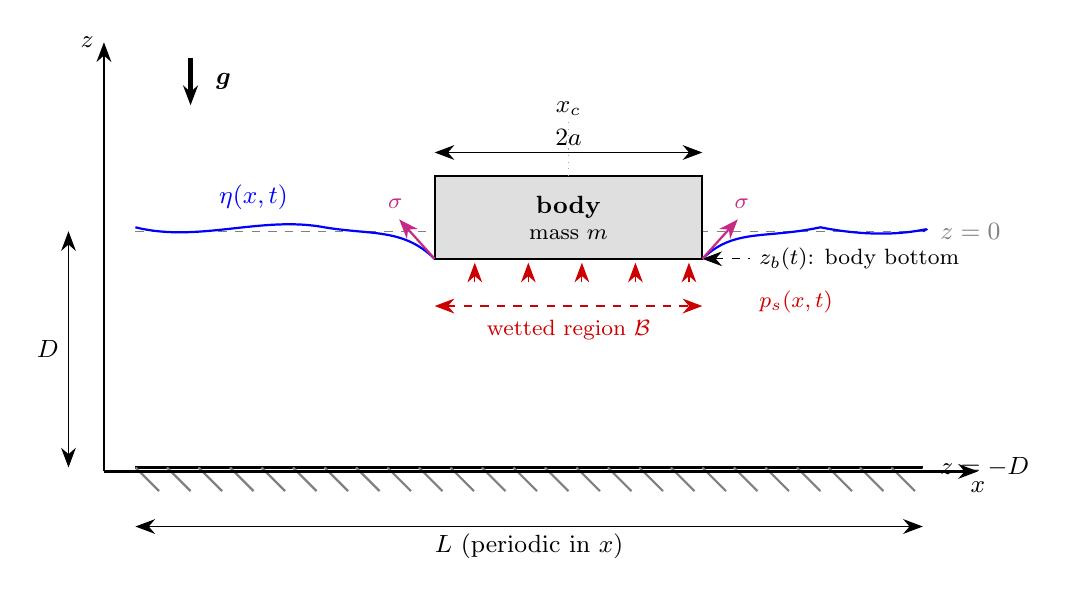
\begin{tikzpicture}[
  >={Stealth[length=2.5mm]},
  font=\small,
  ]

  % Parameters
  \def\Lx{10}
  \def\Dz{3.0}
  \def\Xc{5.5}
  \def\Aw{1.7}
  \def\Zb{0.7}
  \def\Zbot{-0.35}

  % Bottom solid wall (hatched)
  \draw[thick] (0, -\Dz) -- (\Lx, -\Dz);
  \begin{scope}
    \clip (0, -\Dz - 0.35) rectangle (\Lx, -\Dz);
    \foreach \x in {-2, -1.6, ..., 12} {
      \draw[gray, thick] (\x, -\Dz) -- (\x + 0.3, -\Dz - 0.3);
    }
  \end{scope}
  \node[anchor=west] at (\Lx + 0.1, -\Dz) {$z = -D$};

  % Mean surface (dashed)
  \draw[dashed, gray] (0, 0) -- (\Lx, 0);
  \node[anchor=west, gray] at (\Lx + 0.1, 0) {$z = 0$};

  % Free surface eta(x,t)
  \draw[thick, blue]
    (0, 0.05)
    .. controls (0.8, -0.15) and (1.6, 0.2) .. (2.4, 0.05)
    .. controls (3.0, -0.05) and (3.4, 0.04) .. (\Xc - \Aw, \Zbot);
  \draw[thick, blue] (\Xc - \Aw, \Zbot) -- (\Xc + \Aw, \Zbot);
  \draw[thick, blue]
    (\Xc + \Aw, \Zbot)
    .. controls (\Xc + \Aw + 0.4, 0.04) and (\Xc + \Aw + 0.8, -0.1) .. (\Xc + \Aw + 1.5, 0.05)
    .. controls (\Xc + \Aw + 2.5, -0.15) and (\Xc + \Aw + 3.0, 0.1) .. (\Lx, 0);
  \node[blue, anchor=south] at (1.5, 0.15) {$\eta(x, t)$};

  % Body
  \draw[fill=gray!25, thick] (\Xc - \Aw, \Zbot) rectangle (\Xc + \Aw, \Zb);
  \node at (\Xc, \Zb / 2 - 0.05) {\textbf{body}};
  \node[font=\footnotesize] at (\Xc, \Zb / 2 - 0.4) {mass $m$};

  % x_c indicator
  \draw[dotted, gray!70] (\Xc, \Zb) -- (\Xc, \Zb + 0.7);
  \node[anchor=south] at (\Xc, \Zb + 0.65) {$x_c$};

  % 2a label above body
  \draw[<->] (\Xc - \Aw, \Zb + 0.3) -- (\Xc + \Aw, \Zb + 0.3);
  \node[anchor=south] at (\Xc, \Zb + 0.27) {$2a$};

  % z_b indicator
  \draw[<-, dashed] (\Xc + \Aw, \Zbot) -- (\Xc + \Aw + 0.6, \Zbot);
  \node[anchor=west, font=\footnotesize] at (\Xc + \Aw + 0.6, \Zbot)
    {$z_b(t)$: body bottom};

  % Wetted region (below body)
  \draw[<->, thick, dashed, red!80!black] (\Xc - \Aw, \Zbot - 0.6) -- (\Xc + \Aw, \Zbot - 0.6);
  \node[red!80!black, font=\footnotesize] at (\Xc, \Zbot - 0.9) {wetted region $\mathcal{B}$};

  % Surface pressure arrows
  \foreach \fr in {0.15, 0.35, 0.55, 0.75, 0.95} {
    \pgfmathsetmacro{\xa}{\Xc - \Aw + \fr * 2 * \Aw}
    \draw[->, red!80!black, thin] (\xa, \Zbot - 0.3) -- (\xa, \Zbot - 0.05);
  }
  \node[red!80!black, font=\footnotesize, anchor=west] at (\Xc + \Aw + 0.6, \Zbot - 0.55) {$p_s(x, t)$};

  % Contact-line surface tension arrows
  \draw[->, thick, magenta!80!black] (\Xc - \Aw, \Zbot) -- (\Xc - \Aw - 0.45, \Zbot + 0.5);
  \draw[->, thick, magenta!80!black] (\Xc + \Aw, \Zbot) -- (\Xc + \Aw + 0.45, \Zbot + 0.5);
  \node[magenta!80!black, font=\footnotesize] at (\Xc - \Aw - 0.5, \Zbot + 0.7) {$\sigma$};
  \node[magenta!80!black, font=\footnotesize] at (\Xc + \Aw + 0.5, \Zbot + 0.7) {$\sigma$};

  % Domain length L
  \draw[<->] (0, -\Dz - 0.75) -- (\Lx, -\Dz - 0.75);
  \node[anchor=north] at (\Lx/2, -\Dz - 0.72) {$L$ (periodic in $x$)};

  % Domain depth D
  \draw[<->] (-0.85, 0) -- (-0.85, -\Dz);
  \node[anchor=east] at (-0.85, -\Dz/2) {$D$};

  % Gravity arrow
  \draw[->, ultra thick] (0.7, \Zb + 1.5) -- (0.7, \Zb + 0.9);
  \node[anchor=west] at (0.9, \Zb + 1.2) {$\bm{g}$};

  % Axes
  \draw[->, thick] (-0.4, -\Dz - 0.05) -- (\Lx + 0.7, -\Dz - 0.05) node[anchor=north]{$x$};
  \draw[->, thick] (-0.4, -\Dz - 0.05) -- (-0.4, \Zb + 1.7) node[anchor=east]{$z$};

\end{tikzpicture}
\caption{Geometry of the 2D Cartesian floating-body problem.
A flat-bottomed rigid body of half-width $a$ and mass-per-unit-length $m$, centred at $x = x_c$, rests on a viscous fluid layer of depth $D$ in a periodic domain of length $L$.
The free surface $\eta(x, t)$ (blue) deforms continuously outside the wetted region $\mathcal{B}$ and is pinned to the body bottom, $\eta = z_b(t)$, inside $\mathcal{B}$.
The surface pressure $p_s(x, t)$ (red, upward) is supported only on $\mathcal{B}$: it is the Lagrange multiplier that transmits the fluid traction to the body and enforces the no-penetration condition $\partial_z\phi + w^3 = v_b$ on $\mathcal{B}$.
Capillary forces at the two contact lines $x = x_c \pm a$ (magenta) contribute a net vertical lifting force of $2\sigma\sin(\arctan(\eta_x))$ to the body equation of motion (Section~\ref{sec:explicit_traction}).}
\label{fig:schematic_2D}
\end{figure}
\color{black}
\color{blue}
At $t' = 0$ the body is in contact with the fluid surface.
Unlike prescribed-motion formulations, the body motion here is determined self-consistently by Newton's second law driven by gravity and the integrated fluid pressure.
This choice distinguishes the present formulation from a wavemaker-type treatment in which $z_b'(t')$ would be specified in advance: here, both the body trajectory and the fluid response are unknowns of the coupled problem, and the interaction between them is mediated by the surface pressure $p_s'$ on the wetted region of the body.

\paragraph{Body equations of motion.}
The body is a rigid object constrained to move purely vertically; its state is captured by the two scalar fields $z_b(t)$ and $v_b(t)$, the bottom position and vertical velocity.
The body kinematic equation simply identifies $v_b$ as the time derivative of $z_b$,
\begin{equation}
    \frac{\mathrm{d} z_b}{\mathrm{d} t} \;=\; v_b. \label{eq:body_kin}
\end{equation}
Newton's second law applied to the body, in dimensional form, reads
\begin{equation}
    m\,\frac{\mathrm{d} v'_b}{\mathrm{d} t'} \;=\; -m g + \int_{|x' - x_c'| < a'} p'_s(x', t')\,\mathrm{d} x', \label{eq:body_dyn_dim}
\end{equation}
where the left-hand side is the (linear) inertia of the body per unit length, the first term on the right-hand side is its weight, and the integral is the net upward force exerted by the fluid on the body through the wetted region $\mathcal{B}'(t) = \{x' : |x' - x_c'| < a'\}$.
Non-dimensionalising as in Section~\ref{sec:nondim} (using $v_b = v'_b/V_c$, $t = t'/T_c$, $p_s = p'_s/(\rho V_c^2)$, $x_c = x_c'/L_c$, $a = a'/L_c$) and defining the dimensionless mass per unit length
\begin{equation}
    M \;=\; \frac{m}{\rho\,L_c^2}, \label{eq:M_definition}
\end{equation}
equation~\eqref{eq:body_dyn_dim} becomes, after dividing both sides by $\rho V_c^2 L_c$,
\begin{equation}
    M\,\frac{\mathrm{d} v_b}{\mathrm{d} t} \;=\; -\frac{M}{\Fr} + \int_{\mathcal{B}} p_s(x, t)\,\mathrm{d} x. \label{eq:body_dyn}
\end{equation}
\color{black}
The dimensionless weight $-M/\Fr$ reflects the choice of $V_c^2/(g L_c) = \Fr$ as the Froude number~\eqref{eq:dimless}.
(In the summary equations of Section~\ref{sec:model_summary} below, the same dimensionless mass is occasionally written ``$Ma$'' for typographical reasons; the two symbols denote the same quantity.)
Equations~\eqref{eq:body_kin}--\eqref{eq:body_dyn} are the body equations of motion in their Lagrange-multiplier form, in which the integral in~\eqref{eq:body_dyn} is computed from the unknown surface pressure $p_s(x, t)$; an equivalent explicit-traction form is given below in~\eqref{eq:body_dyn_explicit}.

\paragraph{Boundary conditions under the wetted region.}
Let $\mathcal{B}(t) = \{x : |x - x_c| < a\}$ denote the wetted region.
Under $\mathcal{B}$, the free-surface boundary conditions must be replaced because the presence of the solid body renders the interface no longer a free surface: both the location of the interface and the tangential velocity of the fluid there are now constrained by the body geometry and motion.
Three independent conditions are required:
\begin{enumerate}
    \item \emph{Surface follows the body} (geometric constraint):
    \begin{equation}
        \eta(x, t) = z_b(t), \qquad x \in \mathcal{B}(t). \label{eq:body_eta_constraint}
    \end{equation}
    Because the body is rigid and the surface is assumed to remain in contact with its flat bottom, the surface elevation under $\mathcal{B}$ is pinned to the body position.
    This is a kinematic statement about the geometry of the interface, not a dynamic one: it does not by itself determine the body motion.

    \item \emph{Kinematic match} (no-penetration at the body bottom):
    \begin{equation}
        \partial_z \phi + w^3 = v_b(t), \qquad x \in \mathcal{B}(t), \; z = 0. \label{eq:body_kin_match}
    \end{equation}
    The total vertical fluid velocity at the linearised surface, $\partial_z\phi + w^3$, must equal the vertical velocity of the body to prevent interpenetration.
    This replaces the free-surface kinematic condition~\eqref{eq:nd_kin} under the body.
    Its compatibility with~\eqref{eq:body_eta_constraint} follows from differentiating the latter in time: $\partial_t \eta = \dot{z}_b = v_b$, which coincides with~\eqref{eq:nd_kin} evaluated under the body if and only if~\eqref{eq:body_kin_match} holds.
    Thus the two constraints are not redundant but consistent, and together they fully determine the surface motion under the body.

    \item \emph{Horizontal no-slip} at the body bottom:
    \begin{equation}
        \partial_x \phi + w^1 = 0, \qquad x \in \mathcal{B}(t), \; z = 0. \label{eq:body_noslip}
    \end{equation}
    The tangential velocity of the fluid at the body bottom must vanish because the body is rigid and moves only vertically.
    This replaces the surface stress-free condition~\eqref{eq:nd_surf_w1} under the body: a stress-free interface is appropriate at an air--fluid boundary, but not at a solid wall.
\end{enumerate}

\paragraph{Role of the surface pressure.}
The dynamic boundary condition~\eqref{eq:nd_dyn} continues to hold at $z = 0$ everywhere, including under the body.
However, its interpretation changes between the two regions.
Outside $\mathcal{B}$ the surface pressure $p_s$ vanishes (the free surface is in mechanical equilibrium with atmospheric pressure, taken as zero by convention), and~\eqref{eq:nd_dyn} is an evolution equation for $\phi_s$.
Under $\mathcal{B}$ the surface pressure is no longer prescribed: it becomes an unknown whose role is that of a Lagrange multiplier enforcing the kinematic match~\eqref{eq:body_kin_match}.
\color{blue}
From this perspective, $p_s$ under the body represents \emph{whatever pressure distribution the fluid must exert on the bottom of the body} in order to make the fluid velocity match the body velocity at every point.
This interpretation connects naturally to the standard treatment of constrained dynamics in mechanics, where Lagrange multipliers represent the internal forces required to maintain holonomic constraints.

\paragraph{Equivalent explicit-traction form.}
\label{sec:explicit_traction}
Although we treat $p_s$ under $\mathcal{B}$ as an independent unknown, the dynamic boundary condition~\eqref{eq:nd_dyn} (which still holds there) determines it algebraically in terms of the other surface fields.
Solving~\eqref{eq:nd_dyn} for $p_s$ on $\mathcal{B}$,
\begin{equation}
    p_s \;=\; -\partial_t \phi_s - \frac{1}{\Fr}\eta + \frac{1}{\We}\,\partial_{xx}\eta + \frac{2}{\Rey}\,\partial_{xx}\phi_s - \frac{2}{\Rey}\,\partial_z w^3, \label{eq:ps_explicit}
\end{equation}
and substituting~\eqref{eq:ps_explicit} into the body force balance~\eqref{eq:body_dyn}, we recover the body equation of motion in \emph{explicit-traction} form:
\begin{equation}
    M\,\frac{\mathrm{d} v_b}{\mathrm{d} t} \;=\; -\frac{M}{\Fr} + \int_{\mathcal{B}}\!\!\bigg[-\partial_t \phi_s - \frac{1}{\Fr}\eta + \frac{2}{\Rey}\,\partial_{xx}\phi_s - \frac{2}{\Rey}\,\partial_z w^3\bigg]\,\mathrm{d} x + F_\sigma, \label{eq:body_dyn_explicit}
\end{equation}
where the capillary contribution
\begin{equation}
    F_\sigma \;=\; \int_{\mathcal{B}} \frac{1}{\We}\,\partial_{xx}\eta\,\mathrm{d} x \;=\; \frac{1}{\We}\,\big[\partial_x \eta\big]_{x_c - a}^{x_c + a}, \label{eq:F_sigma}
\end{equation}
arises from integrating the curvature term across the wetted region.
Inside the strict interior of $\mathcal{B}$ the surface is flat ($\eta = z_b$, so $\partial_{xx}\eta = 0$), but the surface slope jumps discontinuously at the two contact lines $x = x_c \pm a$; the resulting boundary contribution is, in dimensional form, $\sigma\big[\partial_{x'}\eta'\big]_{x_c'-a'}^{x_c'+a'}$, the vertical projection of the surface-tension pull at the two contact lines.
For a flow that is symmetric about $x = x_c$, the two contact-line contributions add, yielding the form $2\sigma \sin(\arctan(\partial_x \eta))$ that appears in equation~(2.32) of the summary.

The Lagrange-multiplier form~\eqref{eq:body_dyn} and the explicit-traction form~\eqref{eq:body_dyn_explicit} are therefore mathematically equivalent: they yield the same body trajectory and the same fluid response.
Their utility differs in numerical implementation.
In the Lagrange-multiplier form, $p_s$ is an unknown in the linear system and the constraint~\eqref{eq:body_kin_match} appears as an additional row; this is the approach we adopt in Section~\ref{sec:augmented_monolithic}.
\color{black}
In the explicit-traction form, no constraint multiplier is introduced and the body equation is closed by quadrature over the surface fields; the time derivative $\partial_t \phi_s$ that appears in~\eqref{eq:body_dyn_explicit} is then handled implicitly via the surface dynamic equation.
Both approaches admit a one-time LU prefactorisation of the constant-coefficient matrix; the Lagrange-multiplier form was selected here because it produces a sparser block structure and avoids introducing the $\partial_t \phi_s$ coupling explicitly in the body row.

\paragraph{Hydrostatic equilibrium.}
A useful consistency check is to consider the static limit in which the body is at rest on a quiescent fluid ($\dot{v}_b = 0$, $\partial_t \phi_s = 0$, $\ww = 0$).
In this limit, the body equation of motion~\eqref{eq:body_dyn} reduces to the force balance $M/\Fr = \int_{\mathcal{B}} p_s\,\mathrm{d} x$, and the dynamic boundary condition~\eqref{eq:nd_dyn} reduces to $p_s = -\eta/\Fr$ (using $\kappa \to 0$ for a flat surface under the body).
Combining these with the geometric constraint $\eta = z_b$ yields the hydrostatic equilibrium depth
\begin{equation}
    |z_b^{\mathrm{eq}}| = \frac{M}{2a} = \frac{m}{\rho\,\cdot\,2a},
    \label{eq:hydrostatic}
\end{equation}
which is precisely the two-dimensional statement of Archimedes' principle: the body sinks until the displaced fluid mass per unit length equals the body's own mass per unit length.
This result provides a quantitative target for the numerical scheme in Section~\ref{sec:results}.

\paragraph{Summary of the coupled problem.}
The full coupled fluid--body problem thus consists of the bulk fluid equations~\eqref{eq:nd_laplace}--\eqref{eq:nd_heat}, the piecewise-defined surface boundary conditions summarised in Table~\ref{tab:body_bcs}, the body equations of motion~\eqref{eq:body_kin}--\eqref{eq:body_dyn}, and the bottom non-slip conditions~\eqref{eq:nd_bot_w3}--\eqref{eq:nd_bot_w1}.
The additional unknowns introduced by the body are the surface pressure field $p_s(x, t)$ (supported only on $\mathcal{B}$), together with the two scalar body states $z_b(t)$ and $v_b(t)$.

\begin{table}[H]
    \centering
    \caption{Surface boundary conditions as a function of region.  The dynamic condition~\eqref{eq:nd_dyn} applies uniformly, but with $p_s$ prescribed to zero outside the body and left as an unknown inside.}
    \label{tab:body_bcs}
    \begin{tabular}{lll}
        \toprule
        Region & Free surface ($x \notin \mathcal{B}$) & Wetted body ($x \in \mathcal{B}$) \\
        \midrule
        Surface elevation & $\partial_t \eta = \partial_z\phi + w^3$ & $\eta = z_b$ \\
        Kinematic & (evolves $\eta$) & $\partial_z\phi + w^3 = v_b$ \\
        Horizontal vortical $w^1$ & $\partial_z w^1 = -(\partial_{xz}\phi + \partial_x w^3)$ & $\partial_x\phi + w^1 = 0$ \\
        Surface pressure & $p_s = 0$ & $p_s$ unknown \\
        \bottomrule
    \end{tabular}
\end{table}

\color{blue}
\subsection{Extension to axisymmetric coordinates}
\label{sec:axisymm}

The two-dimensional Cartesian model of Sections~\ref{sec:setup}--\ref{sec:floating_body} generalises naturally to axisymmetric cylindrical coordinates $(r, z)$, in which the flow is independent of the azimuthal angle and the body becomes a flat-bottomed cylinder (a disk-bottomed solid) sitting on the surface.
This is the natural setting for three-dimensional rigid bodies centred on the symmetry axis (centred drops, disks, plates), and it is the geometry of the original sphere-impact problem of \citet{GaleanoRiosEtAl2017} in the appropriate flat-bottom limit.
The axisymmetric geometry is illustrated in Figure~\ref{fig:schematic_axi}.

\begin{figure}[H]
\centering

\begin{minipage}[t]{0.56\textwidth}
\centering
\textbf{(a) Computational $(r, z)$ cross-section}\\[0.4em]
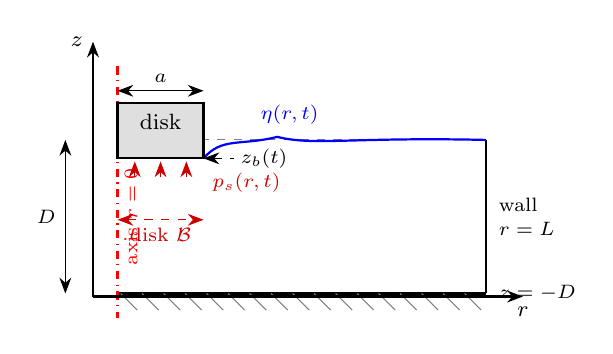
\begin{tikzpicture}[
  >={Stealth[length=2mm]},
  font=\footnotesize,
  scale=0.78,
  ]
  \def\Lx{6}
  \def\Dz{2.5}
  \def\Aw{1.4}
  \def\Zb{0.6}
  \def\Zbot{-0.3}

  % Bottom solid wall
  \draw[thick] (0, -\Dz) -- (\Lx, -\Dz);
  \begin{scope}
    \clip (0, -\Dz - 0.3) rectangle (\Lx, -\Dz);
    \foreach \x in {-1, -0.65, ..., 8} {
      \draw[gray] (\x, -\Dz) -- (\x + 0.27, -\Dz - 0.27);
    }
  \end{scope}
  \node[anchor=west, font=\scriptsize] at (\Lx + 0.05, -\Dz) {$z = -D$};

  % Outer wall (solid line)
  \draw[thick] (\Lx, 0) -- (\Lx, -\Dz);
  \node[anchor=west, font=\scriptsize] at (\Lx + 0.05, -\Dz/2 + 0.2) {wall};
  \node[anchor=west, font=\scriptsize] at (\Lx + 0.05, -\Dz/2 - 0.2) {$r = L$};

  % Axis of symmetry (dash-dot, red, at r=0)
  \draw[dash dot, thick, red] (0, \Zb + 0.6) -- (0, -\Dz - 0.4);
  \node[red, rotate=90, anchor=north, font=\scriptsize] at (-0.05, -\Dz/2) {axis $r = 0$};

  % Mean surface (dashed)
  \draw[dashed, gray] (0, 0) -- (\Lx, 0);

  % Free surface eta(r,t): flat under body, wavy outside
  \draw[thick, blue] (0, \Zbot) -- (\Aw, \Zbot);
  \draw[thick, blue]
    (\Aw, \Zbot)
    .. controls (\Aw + 0.3, 0.05) and (\Aw + 0.6, -0.1) .. (\Aw + 1.2, 0.05)
    .. controls (\Aw + 1.8, -0.1) and (\Aw + 2.4, 0.05) .. (\Lx, 0);
  \node[blue, anchor=south, font=\scriptsize] at (\Aw + 1.4, 0.1) {$\eta(r, t)$};

  % Disk body (cross-section: rectangle 0..a)
  \draw[fill=gray!25, thick] (0, \Zbot) rectangle (\Aw, \Zb);
  \node at (\Aw/2, \Zb/2) {disk};

  % radius a label above body
  \draw[<->] (0, \Zb + 0.2) -- (\Aw, \Zb + 0.2);
  \node[anchor=south, font=\scriptsize] at (\Aw/2, \Zb + 0.17) {$a$};

  % z_b label
  \draw[<-, dashed] (\Aw, \Zbot) -- (\Aw + 0.5, \Zbot);
  \node[anchor=west, font=\scriptsize] at (\Aw + 0.45, \Zbot) {$z_b(t)$};

  % p_s arrows
  \foreach \fr in {0.2, 0.5, 0.8} {
    \pgfmathsetmacro{\xa}{\fr * \Aw}
    \draw[->, red!80!black, thin] (\xa, \Zbot - 0.3) -- (\xa, \Zbot - 0.05);
  }
  \node[red!80!black, font=\scriptsize] at (\Aw + 0.7, \Zbot - 0.4) {$p_s(r, t)$};

  % Wetted disk
  \draw[<->, dashed, red!80!black] (0, \Zbot - 1.0) -- (\Aw, \Zbot - 1.0);
  \node[red!80!black, font=\scriptsize] at (\Aw/2, \Zbot - 1.25) {disk $\mathcal{B}$};

  % Depth D
  \draw[<->] (-0.85, 0) -- (-0.85, -\Dz);
  \node[anchor=east, font=\scriptsize] at (-0.85, -\Dz/2) {$D$};

  % Axes
  \draw[->, thick] (-0.4, -\Dz - 0.05) -- (\Lx + 0.6, -\Dz - 0.05) node[anchor=north]{$r$};
  \draw[->, thick] (-0.4, -\Dz - 0.05) -- (-0.4, \Zb + 1.0) node[anchor=east]{$z$};
\end{tikzpicture}
\end{minipage}\hfill%
\begin{minipage}[t]{0.42\textwidth}
\centering
\textbf{(b) 3D perspective}\\[0.4em]
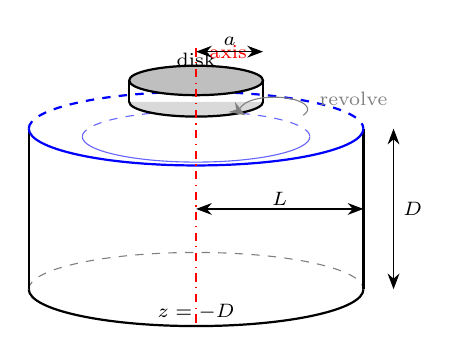
\begin{tikzpicture}[
  >={Stealth[length=2mm]},
  font=\footnotesize,
  scale=0.85,
  ]
  % Cylindrical fluid domain
  % top ellipse (mean surface)
  \draw[dashed, gray] (-2.5, 0) arc (180:360:2.5 and 0.55);
  \draw[dashed, gray] (-2.5, 0) arc (180:0:2.5 and 0.55);
  % bottom ellipse (z = -D)
  \draw[thick] (-2.5, -2.4) arc (180:360:2.5 and 0.55);
  \draw[dashed, gray] (-2.5, -2.4) arc (180:0:2.5 and 0.55);
  % cylinder sides
  \draw[thick] (-2.5, 0) -- (-2.5, -2.4);
  \draw[thick] (2.5, 0) -- (2.5, -2.4);

  % Wavy axisymmetric surface (show as nested rings of varying depth)
  \draw[thick, blue] (-2.5, 0) arc (180:360:2.5 and 0.55);
  \draw[thick, blue, dashed] (-2.5, 0) arc (180:0:2.5 and 0.55);
  % An inner ring suggesting a wave crest
  \draw[blue!60, smooth] (-1.7, -0.12) arc (180:360:1.7 and 0.38);
  \draw[blue!60, dashed, smooth] (-1.7, -0.12) arc (180:0:1.7 and 0.38);

  % Disk body (top): two ellipses + sides
  % Disk body: radius 1.0, thickness 0.32, bottom at z = +0.4 (partially submerged visually)
  % bottom edge of disk
  \draw[fill=gray!30, thick] (-1.0, 0.4) arc (180:360:1.0 and 0.22);
  % side edges
  \draw[thick] (-1.0, 0.4) -- (-1.0, 0.72);
  \draw[thick] (1.0, 0.4) -- (1.0, 0.72);
  % top of disk
  \draw[fill=gray!50, thick] (-1.0, 0.72) arc (180:360:1.0 and 0.22)
        -- (1.0, 0.72) arc (0:180:1.0 and 0.22) -- cycle;
  \node[font=\scriptsize, anchor=south] at (0, 0.78) {disk};

  % Axis of symmetry through center
  \draw[dash dot, thick, red] (0, -2.9) -- (0, 1.2);
  \node[red, anchor=west, font=\scriptsize] at (0.05, 1.15) {axis};

  % Disk radius arrow
  \draw[<->, font=\scriptsize] (0, 1.15) -- (1.0, 1.15);
  \node[anchor=south, font=\scriptsize] at (0.5, 1.1) {$a$};

  % L radius indicator
  \draw[<->, font=\scriptsize] (0, -1.2) -- (2.5, -1.2);
  \node[anchor=south, font=\scriptsize] at (1.25, -1.3) {$L$};

  % Depth D
  \draw[<->, font=\scriptsize] (2.95, 0) -- (2.95, -2.4);
  \node[anchor=west, font=\scriptsize] at (2.95, -1.2) {$D$};

  % bottom label
  \node[anchor=south, font=\scriptsize] at (0, -3) {$z = -D$};

  % "revolves about axis" hint
  \draw[->, gray] (1.6, 0.2) arc (-30:210:0.5 and 0.18);
  \node[gray, font=\scriptsize, anchor=west] at (1.7, 0.45) {revolve};
\end{tikzpicture}
\end{minipage}

\caption{Geometry of the axisymmetric floating-body problem (Section~\ref{sec:axisymm}).
\textbf{(a)} Computational $(r, z)$ cross-section in the half-plane $r \ge 0$.
The symmetry axis $r = 0$ (red dash-dot) carries Neumann mirror conditions for even fields $\phi, \eta, w^z$ and the vanishing $w^r(0) = 0$ from regularity of the odd radial field.
The outer wall $r = L$ closes the domain with Dirichlet zero on all fields, which acts as a strict non-slip wall provided $L$ is large enough that surface waves have decayed before reaching it.
The disk of radius $a$ sits at $z = z_b(t)$ above the bottom $z = -D$; the wetted region $\mathcal{B} = \{r : r < a\}$ supports the surface pressure $p_s(r, t)$ (red arrows).
\textbf{(b)} Three-dimensional perspective obtained by revolving (a) about the symmetry axis: a cylindrical fluid of radius $L$ and depth $D$ with a flat-bottomed disk body of radius $a$ on top.
The integration weight appearing in Newton's law is the cylindrical area element $2\pi r\,\mathrm{d} r$ (Section~\ref{sec:axisymm_body}), so the body mass per disk area is naturally $m/(\pi a^2)$ in equilibrium.}
\label{fig:schematic_axi}
\end{figure}

\subsubsection{Axisymmetric operators}
\label{sec:axisymm_ops}

For a scalar field $\phi(r, z, t)$ with no azimuthal dependence, the three-dimensional Laplacian becomes
\begin{equation}
    \Delta\phi \;=\; \partial_{rr}\phi + \frac{1}{r}\,\partial_r\phi + \partial_{zz}\phi
              \;\equiv\; \Delta_{\mathrm{ax}}\phi.
    \label{eq:laplacian_axi}
\end{equation}
The radial part of \eqref{eq:laplacian_axi},
\begin{equation}
    \Delta_{H,\mathrm{ax}} \;:=\; \partial_{rr} + \frac{1}{r}\,\partial_r,
    \label{eq:Delta_H_axi_def}
\end{equation}
is the natural axisymmetric analogue of $\partial_{xx}$ in the two-dimensional Cartesian setting: it is the operator appearing in the surface dynamic condition~\eqref{eq:nd_dyn} (with $\partial_{xx}\eta$ and $\partial_{xx}\phi_s$ replaced by $\Delta_{H,\mathrm{ax}}\eta$ and $\Delta_{H,\mathrm{ax}}\phi_s$) and the surface vorticity equation~\eqref{eq:nd_vort}.

For vector quantities with a radial component, the Laplacian acquires an extra contribution arising from the curvature of the cylindrical basis.
For the radial vortical component $w^r$, the vector Laplacian reads
\begin{equation}
    (\Delta \ww)^r \;=\; \Delta_{\mathrm{ax}}\, w^r \;-\; \frac{w^r}{r^2},
    \label{eq:vector_laplacian_wr}
\end{equation}
the extra $-w^r/r^2$ reflecting the fact that an axisymmetric radial field is odd in $r$ and must vanish at $r = 0$.
This term is essential: omitting it would make the bulk heat equation for $w^r$ inconsistent at small $r$.

\subsubsection{Axis and outer-wall boundary conditions}
\label{sec:axisymm_BCs}

Two boundary conditions specific to the axisymmetric problem arise in addition to those of Sections~\ref{sec:bc_free_surface}--\ref{sec:stress_free_w1}.

\paragraph{Axis regularity ($r = 0$).}
The scalar fields $\phi$, $\eta$, $w^z$ are even in $r$, giving Neumann (mirror) boundary conditions $\partial_r \phi|_{r=0} = 0$ and similarly for $\eta$ and $w^z$.
The radial vector field $w^r$ is odd in $r$, hence $w^r(0) = 0$ by regularity.
At $r = 0$ the operator $\Delta_{H,\mathrm{ax}}$ exhibits the apparent singularity $(1/r)\partial_r f$; applying L'H\^opital's rule together with the mirror condition yields the finite limit
\begin{equation}
    \lim_{r \to 0^+}\left(\partial_{rr} f + \frac{1}{r}\,\partial_r f\right) \;=\; 2\,\partial_{rr} f\big|_{r=0},
    \label{eq:Lhopital_axis}
\end{equation}
which after the centred discrete mirror condition $f_{-1} = f_1$ collapses to the stencil
\begin{equation}
    (\bm{\Delta}_{H,\mathrm{ax}} f)_0 \;=\; \frac{4\,(f_1 - f_0)}{(\Delta r)^2}.
    \label{eq:Delta_H_axi_at_axis}
\end{equation}

\paragraph{Outer-wall closure ($r = L$).}
The radial domain is finite by necessity.
We pick $L$ large enough that the surface waves emitted by the body do not reach $r = L$ within the simulation time (or, equivalently, that wave amplitudes have decayed to negligible levels by that radius).
At $r = L$ we impose Dirichlet zero on all fields, $\phi = w^z = w^r = \eta = 0$, which is the natural ``effectively infinite'' boundary condition.
Because $\phi = 0$ holds along the entire wall, $\partial_z \phi = 0$ there too, so $\uu = \nabla\phi + \ww = \bm{0}$ on the wall: the Dirichlet closure IS a strict non-slip wall in the far-wall limit.
This is the radial analogue of the periodic-in-$x$ closure used in Section~\ref{sec:setup}; both are ``spend domain size to save boundary complexity'' strategies.

\subsubsection{Axisymmetric floating body}
\label{sec:axisymm_body}

For a rigid flat-bottomed cylinder of radius $a$ and mass $m$, with vertical position $z_b(t)$ constrained to vertical motion by axisymmetry, the wetted region is the disk $\mathcal{B} = \{r : r < a\}$.
The geometric, kinematic-match, and horizontal-no-slip conditions of \eqref{eq:body_eta_constraint}--\eqref{eq:body_noslip} carry over identically with $x \to r$ and $w^1 \to w^r$:
\begin{align}
    \eta(r, t) \;&=\; z_b(t),                                & r \in \mathcal{B}, \label{eq:body_eta_axi} \\
    \partial_z \phi + w^z \;&=\; v_b(t),                     & r \in \mathcal{B},\; z = 0, \label{eq:body_kin_axi} \\
    \partial_r \phi + w^r \;&=\; 0,                          & r \in \mathcal{B},\; z = 0. \label{eq:body_noslip_axi}
\end{align}

Newton's second law for the body now involves the cylindrical area element $2\pi r\,\mathrm{d} r$.
In dimensional form,
\begin{equation}
    m\,\frac{\mathrm{d} v'_b}{\mathrm{d} t'} \;=\; -m\,g + \int_0^{a'} p'_s(r', t')\,2\pi r'\,\mathrm{d} r'. \label{eq:body_newton_axi_dim}
\end{equation}
Non-dimensionalising as in Section~\ref{sec:nondim} with the \emph{three-dimensional} mass scaling
\begin{equation}
    M \;=\; \frac{m}{\rho\,L_c^{\,3}}, \label{eq:M_axi_def}
\end{equation}
gives the dimensionless body equation
\begin{equation}
    M\,\frac{\mathrm{d} v_b}{\mathrm{d} t} \;=\; -\frac{M}{\Fr} + \int_0^{a} p_s(r, t)\,2\pi r\,\mathrm{d} r. \label{eq:body_newton_axi}
\end{equation}
The integrand $p_s(r)\cdot 2\pi r$ is the cylindrical area element; its appearance distinguishes axisymmetric integration from the 1D Cartesian integration of Section~\ref{sec:floating_body}.
The mass scaling~\eqref{eq:M_axi_def} also differs from the 2D Cartesian $M = m/(\rho L_c^{\,2})$ used in Section~\ref{sec:floating_body}: in axisymmetric coordinates~$M$ is a genuinely three-dimensional dimensionless mass.

\paragraph{3D Archimedes equilibrium.}
At hydrostatic equilibrium ($\dot v_b = 0$, $\partial_t \phi_s = 0$, $\ww = 0$), the dynamic boundary condition under the body reduces to $p_s = -z_b/\Fr$ (constant in $r$, since $\eta = z_b$ is uniform on $\mathcal{B}$ and capillary contributions concentrate at the contact line).
Substituting into~\eqref{eq:body_newton_axi}, the force balance gives
\begin{equation}
    \frac{M}{\Fr} \;=\; \int_0^{a}\!\!\left(-\frac{z_b}{\Fr}\right) 2\pi r\,\mathrm{d} r \;=\; -\frac{z_b\,\pi a^2}{\Fr},
\end{equation}
yielding the three-dimensional Archimedes principle
\begin{equation}
    \boxed{\;|z_b^{\mathrm{eq}}| \;=\; \frac{M}{\pi a^2} \;=\; \frac{m}{\rho\,\pi a^2}\;.\;}
    \label{eq:Archimedes_3D}
\end{equation}
The disk area $\pi a^2$ replaces the 1D Cartesian footprint $2a$ of equation~\eqref{eq:hydrostatic}.
A release-from-rest test at $z_b(0) = 0$, $v_b(0) = 0$ should produce a damped oscillation about $z_b = -M/(\pi a^2)$, decaying toward this equilibrium under viscous damping.
This is the quantitative validation target for the axisymmetric implementation.
\color{black}


%% ================================================================
%% 3. NUMERICAL METHODS
%% ================================================================
\section{Numerical methods}
\label{sec:numerical}

\subsection{Spatial discretisation}
\label{sec:spatial}

We discretise the domain on a uniform rectangular grid with $n_x$ points in $x$ and $n_z$ points in $z$:
\begin{equation}
    x_j = j\,\Delta x, \quad j = 0, \ldots, n_x - 1; \qquad
    z_i = -D + i\,\Delta z, \quad i = 0, \ldots, n_z - 1,
\end{equation}
with $\Delta x = L/n_x$ and $\Delta z = D/(n_z - 1)$.
The index $i = 0$ corresponds to the bottom ($z = -D$) and $i = n_z - 1$ to the free surface ($z = 0$).
\color{blue}
For any grid function $u_{i,j}$ defined on this mesh we use the shorthand $u_j^{\mathrm{s}} := u_{n_z-1, j}$ for the surface trace, $u_j^{\mathrm{b}} := u_{0, j}$ for the bottom trace, and $u^{n}_{i,j}$ for the value at time level $n$.

\subsubsection{Discrete horizontal operators}

The horizontal grid is periodic, so the discrete horizontal Laplacian $\bm{\Delta}_H \in \mathbb{R}^{n_x \times n_x}$ has entries
\begin{equation}
    (\bm{\Delta}_H)_{jk} \;=\; \frac{1}{(\Delta x)^2}\,\big[\,\delta_{k,\,j-1 \,\mathrm{mod}\, n_x} \;-\; 2\,\delta_{kj} \;+\; \delta_{k,\,j+1\,\mathrm{mod}\, n_x}\,\big], \label{eq:Delta_H_entries}
\end{equation}
giving the standard second-order three-point stencil
\begin{equation}
    (\bm{\Delta}_H u)_j \;=\; \frac{u_{j+1} - 2 u_j + u_{j-1}}{(\Delta x)^2}, \qquad j \pm 1 \equiv (j\pm 1)\,\mathrm{mod}\, n_x. \label{eq:Delta_H_stencil}
\end{equation}
The centred first-derivative operator $\bm{D}_x \in \mathbb{R}^{n_x \times n_x}$ has entries
\begin{equation}
    (\bm{D}_x)_{jk} \;=\; \frac{1}{2\Delta x}\,\big[\,\delta_{k,\,j+1\,\mathrm{mod}\, n_x} \;-\; \delta_{k,\,j-1\,\mathrm{mod}\, n_x}\,\big], \label{eq:Dx_entries}
\end{equation}
i.e.\ $(\bm{D}_x u)_j = (u_{j+1} - u_{j-1})/(2\Delta x)$.
Both operators are second-order accurate in $\Delta x$, and both are circulant: they commute with each other and admit a closed-form spectrum via discrete Fourier modes, although we do not exploit this here---we simply assemble them as sparse \texttt{csr} matrices and pass them to a direct LU solver.

\subsubsection{Discrete vertical operators}

For derivatives in $z$, we use centred differences at interior nodes and one-sided differences at the boundaries.
The interior centred second derivative is
\begin{equation}
    (\bm{T}_z u)_{i,j} \;=\; \frac{u_{i+1,j} - 2 u_{i,j} + u_{i-1,j}}{(\Delta z)^2}, \qquad 1 \le i \le n_z - 2, \label{eq:dzz_interior}
\end{equation}
and the centred first derivative is $(\bm{D}_z u)_{i,j} = (u_{i+1,j} - u_{i-1,j})/(2\Delta z)$.
At the boundaries we use the one-sided forward and backward differences
\begin{align}
    (\bm{D}_z u)_{0,j} \;&=\; \frac{u_{1,j} - u_{0,j}}{\Delta z}, \label{eq:dz_bottom} \\
    (\bm{D}_z u)_{n_z-1,j} \;&=\; \frac{u_{n_z-1,j} - u_{n_z-2,j}}{\Delta z}, \label{eq:dz_surface}
\end{align}
each of which is first-order accurate in $\Delta z$.
The use of one-sided stencils at $i = 0$ and $i = n_z - 1$ is dictated by the structure of the boundary conditions: the surface kinematic~\eqref{eq:nd_kin}, dynamic~\eqref{eq:nd_dyn} and stress-free~\eqref{eq:nd_surf_w1} conditions all involve $\partial_{z}\phi$ or $\partial_{z} w^3$ evaluated at $z = 0$ from below, and similarly the bottom non-slip conditions~\eqref{eq:nd_bot_w3}--\eqref{eq:nd_bot_w1} involve $\partial_{z}\phi$ at $z = -D$ from above.
A centred stencil at these boundary rows would require ghost-point values that the discrete operator has no natural way of producing.

\subsubsection{Discrete 2D Laplacian}

The two-dimensional Laplacian on the rectangular grid is constructed by the tensor-product (Kronecker) sum
\begin{equation}
    \bm{\Delta}_{2\mathrm{D}} \;=\; \bm{I}_{n_z} \otimes \bm{\Delta}_H \;+\; \bm{T}_z \otimes \bm{I}_{n_x}, \label{eq:Delta_2D}
\end{equation}
where $\bm{T}_z \in \mathbb{R}^{n_z \times n_z}$ is the one-dimensional second-derivative operator in $z$, with entries~\eqref{eq:dzz_interior} on interior rows.
The boundary rows of $\bm{T}_z$ are not used in~\eqref{eq:Delta_2D} as-is: when assembling the heat-equation block of the monolithic matrix (Section~\ref{sec:monolithic}), the rows $i = 0$ and $i = n_z - 1$ are overwritten by the corresponding boundary conditions (the bottom non-slip~\eqref{eq:nd_bot_w3} or surface vorticity~\eqref{eq:nd_vort} for the $w^3$ block, and analogously for the $w^1$ and $\phi$ blocks).
The Kronecker structure renders $\bm{\Delta}_{2\mathrm{D}}$ banded with at most five nonzero entries per row in the interior; the resulting sparsity is preserved through the LU factorisation, with fill-in bounded by the bandwidth $n_x$.
\color{black}

\subsection{Sequential solver}
\label{sec:sequential}

The sequential solver advances the solution from time level $n$ to $n+1$ in four sub-steps, each involving one or more sparse linear solves.
\color{blue}
For the time discretisation we adopt the (first-order) implicit Euler scheme, which is unconditionally stable for the bulk heat equation and for the surface diffusion operator $(I - 2\Delta t/\Rey)\,\bm{\Delta}_H$.
Unconditional stability is essential here because the surface vorticity equation~\eqref{eq:nd_vort} introduces a horizontal diffusion coefficient $2/\Rey$ that, when combined with the spatial grid size $\Delta x$, would impose the stiff explicit CFL constraint $\Delta t \le \Rey\,(\Delta x)^2/4$ for an explicit time stepping; with $n_x = 300$ and $\Rey \sim 10^3$, that bound is in the range of $10^{-7}$~s, much smaller than the wave period of interest.
Implicit Euler trades a slightly more expensive linear solve at each step for the freedom to set $\Delta t$ by accuracy rather than stability.

The generic implicit-Euler discretisation of an evolution equation $\partial_t u = \mathcal{L}\, u + f$, with linear operator $\mathcal{L}$ and forcing $f$, reads
\begin{equation}
    \frac{u^{n+1} - u^n}{\Delta t} \;=\; \mathcal{L}\, u^{n+1} + f^{n}, \qquad \Longleftrightarrow \qquad (\bm{I} - \Delta t\,\bm{\mathcal{L}})\,u^{n+1} \;=\; u^n + \Delta t\,f^n, \label{eq:implicit_euler_template}
\end{equation}
where $\bm{\mathcal{L}}$ is the discrete operator approximating $\mathcal{L}$ on the grid.
Each of the four steps below is an instance of~\eqref{eq:implicit_euler_template} applied to one of the bulk or surface equations of Section~\ref{sec:nondim}.
\color{black}

\paragraph{Step 1: Evolve $w^3$ and $w^1$ (heat equations).}
The bulk heat equation~\eqref{eq:nd_heat} is discretised implicitly:
\begin{equation}
    \left(I - \frac{\Delta t}{\Rey}\,\Delta_{2\text{D}}\right) w^{i,n+1} = w^{i,n}, \quad i = 1, 3,
    \label{eq:heat_implicit}
\end{equation}
where $\Delta_{2\text{D}}$ is the discrete 2D Laplacian.
After solving the bulk, the boundary conditions are overwritten:

\begin{itemize}
    \item \emph{Bottom} ($i = 0$): $w^{3,n+1}_j = -(\phi^n_{1,j} - \phi^n_{0,j})/\Delta z$ and $w^{1,n+1}_j = -(D_x\,\phi^n_0)_j$, where $D_x$ is the centred difference operator in $x$.
    \item \emph{Surface} ($i = n_z - 1$) \emph{for} $w^3$: equation~\eqref{eq:nd_vort} discretised implicitly,
    \begin{equation}
        \left(I - \frac{2\Delta t}{\Rey}\,\Delta_H\right) w^{3,n+1}_s = w^{3,n}_s + \frac{2\Delta t}{\Rey}\,\Delta_H\,\phi_z^n, \label{eq:w3_surf_disc}
    \end{equation}
    where $\phi_z^n = (\phi^n_{n_z-1} - \phi^n_{n_z-2})/\Delta z$.
    \item \emph{Surface for} $w^1$: stress-free condition~\eqref{eq:nd_surf_w1} discretised as $w^1_{n_z-1} = w^1_{n_z-2} - \Delta z\,(\phi_{xz}^n + D_x\,w^{3,n+1}_s)$.
\end{itemize}

\paragraph{Step 2: Update surface potential $\phi_s$ (dynamic condition).}
Equation~\eqref{eq:nd_dyn} is discretised implicitly in the diffusion term:
\begin{equation}
    \left(I - \frac{2\Delta t}{\Rey}\,\Delta_H\right) \phi_s^{n+1} = \phi_s^n - \frac{\Delta t}{\Fr}\,\eta^n + \frac{\Delta t}{\We}\,\kappa[\eta^n] - \frac{2\Delta t}{\Rey}\,(D_z\,w^{3,n+1})_s,
    \label{eq:phi_s_disc}
\end{equation}
where $\kappa[\eta] = \Delta_H\eta$ (linearised curvature) and $(D_z\,w^3)_s = (w^3_{n_z-1} - w^3_{n_z-2})/\Delta z$.

\paragraph{Step 3: Solve Laplace equation for bulk $\phi$.}
With the updated surface Dirichlet condition $\phi_{n_z-1,j} = (\phi_s)_j^{n+1}$ and the bottom ghost-point condition enforcing $\partial_z\phi = -w^{3,n+1}_0$ (from~\eqref{eq:nd_bot_w3}), we solve:
\begin{equation}
    A_{\text{Lap}}\,\vec{\phi}^{n+1} = \vec{b}_{\text{Lap}}, \label{eq:laplace_disc}
\end{equation}
where $A_{\text{Lap}}$ encodes the five-point Laplacian with periodic horizontal and appropriate vertical boundary conditions.

\paragraph{Step 4: Update surface elevation $\eta$ (kinematic condition).}
Equation~\eqref{eq:nd_kin} is updated explicitly:
\begin{equation}
    \eta^{n+1} = \eta^n + \Delta t\,\left(\phi_z^{n+1} + w^{3,n+1}_s\right), \label{eq:eta_disc}
\end{equation}
where $\phi_z^{n+1} = (\phi^{n+1}_{n_z-1} - \phi^{n+1}_{n_z-2})/\Delta z$.

Each time step thus requires solving: two $n_z n_x$-sized heat systems (for $w^3$ and $w^1$), two $n_x$-sized tridiagonal-like surface systems (for $w^3_s$ and $\phi_s$), and one $n_z n_x$-sized Laplace system.
\color{blue}
The sequential approach is conceptually simple but suffers from two drawbacks.
First, each of the five sparse solves must be performed at every time step, and although individual solves are cheap on a moderate grid, the call overhead of \texttt{scipy.sparse.linalg.spsolve} dominates the wall-clock cost.
Second, the explicit lagging of the $\phi^n_{xz}$ term in the stress-free boundary update for $w^1$ at the surface (Step~1, last bullet) introduces a small but measurable error that vanishes only as $\Delta t \to 0$.
Both drawbacks are eliminated in the monolithic formulation of Section~\ref{sec:monolithic}, in which all five blocks are assembled into a single linear system, the surface stress-free condition is imposed simultaneously with all other coupling, and the matrix is factored once via sparse LU decomposition.
\color{black}

\subsection{Monolithic formulation}
\label{sec:monolithic}

The sequential solver calls \texttt{spsolve} multiple times per step.
We now show that the entire system can be assembled into a single matrix equation.

\subsubsection{Unknown vector}

The full state at time level $n+1$ is collected into a single vector:
\begin{equation}
    \xx = \begin{pmatrix} \vec{w}^3 \\ \vec{w}^1 \\ \vec{\phi}_s \\ \vec{\phi}_{\mathrm{bulk}} \\ \vec{\eta} \end{pmatrix}, \qquad N_{\mathrm{total}} = 3\,n_z n_x + 2\,n_x.
    \label{eq:state_vector}
\end{equation}

\subsubsection{Block structure}

The monolithic system $A\,\xx^{n+1} = \bb(\xx^n)$ has a block lower-triangular structure:

\begin{center}
\begin{tabular}{lcccccl}
\toprule
Row block & $w^3$ & $w^1$ & $\phi_s$ & $\phi_{\mathrm{bulk}}$ & $\eta$ & Equation \\
\midrule
$w^3$             & $\bullet$ &           &             &                &        & Heat eq.\ + BCs \\
$w^1$             & $\bullet$ & $\bullet$ &             &                &        & Heat eq.\ + BCs \\
$\phi_s$          & $\bullet$ &           & $\bullet$   &                &        & Dynamic BC~\eqref{eq:nd_dyn} \\
$\phi_{\mathrm{bulk}}$ & $\bullet$ &     & $\bullet$   & $\bullet$      &        & Laplace eq. \\
$\eta$            & $\bullet$ &           &             & $\bullet$      & $\bullet$ & Kinematic BC~\eqref{eq:nd_kin} \\
\bottomrule
\end{tabular}
\end{center}

The block lower-triangular structure arises because:
\begin{itemize}
    \item The $w^3$ block depends only on $w^{3,n+1}$ (implicitly) and $\phi^n$ (explicitly, in the RHS).
    \item The $w^1$ block depends on $w^{1,n+1}$ and $w^{3,n+1}$ (through the stress-free surface BC).
    \item The $\phi_s$ block depends on $\phi_s^{n+1}$ and $w^{3,n+1}$ (through $\partial_z w^3$).
    \item The Laplace block depends on $\phi_{\mathrm{bulk}}^{n+1}$, $\phi_s^{n+1}$ (Dirichlet top), and $w^{3,n+1}$ (ghost point at bottom).
    \item The $\eta$ block depends on $\eta^{n+1}$, $\phi_{\mathrm{bulk}}^{n+1}$ (through $\phi_z$), and $w^{3,n+1}_s$.
\end{itemize}

\color{blue}
\subsubsection{Row-by-row specification of \texorpdfstring{$A$}{A}}
\label{sec:row_by_row}

For concreteness we now write out the rows of $A$ explicitly, for each block.
Let $c_x = 1/(\Delta x)^2$, $c_z = 1/(\Delta z)^2$, $\alpha_{\Rey} = \Delta t/\Rey$, $\beta_{\Rey} = 2\Delta t/\Rey$; let $j_{\mathrm{L}} = (j - 1)\,\mathrm{mod}\, n_x$ and $j_{\mathrm{R}} = (j + 1)\,\mathrm{mod}\, n_x$ denote the periodic neighbours of column~$j$.
We index unknowns by $(\mathrm{block}, i, j)$ where the block specifies which field, $i \in \{0,\dots,n_z-1\}$ is the vertical level, and $j \in \{0,\dots,n_x-1\}$ is the horizontal node.
The components of~$\xx$ are stored in the order $\bm{w}^3$, $\bm{w}^1$, $\bm{\phi}_s$, $\bm{\phi}_{\mathrm{bulk}}$, $\bm{\eta}$.

\paragraph{$w^3$ block.}
For interior rows $1 \le i \le n_z - 2$, the implicit-Euler heat equation~\eqref{eq:heat_implicit} gives
\begin{equation}
    \big[1 + 2\alpha_{\Rey}(c_x + c_z)\big]\,w^{3,n+1}_{i,j} \;-\; \alpha_{\Rey} c_x\,(w^{3,n+1}_{i, j_{\mathrm{L}}} + w^{3,n+1}_{i, j_{\mathrm{R}}}) \;-\; \alpha_{\Rey} c_z\,(w^{3,n+1}_{i-1, j} + w^{3,n+1}_{i+1, j}) \;=\; w^{3,n}_{i,j}. \label{eq:w3_interior_row}
\end{equation}
On the bottom row ($i = 0$), the non-slip condition~\eqref{eq:bc_bot_w3} written with the forward difference~\eqref{eq:dz_bottom} yields the linear constraint
\begin{equation}
    w^{3,n+1}_{0, j} \;+\; \frac{1}{\Delta z}\big(\phi^{n+1}_{1, j} - \phi^{n+1}_{0, j}\big) \;=\; 0. \label{eq:w3_bottom_row}
\end{equation}
On the surface row ($i = n_z - 1$), the implicit-Euler discretisation of the surface vorticity equation~\eqref{eq:nd_vort} gives
\begin{equation}
    \big[1 + 2\beta_{\Rey} c_x\big]\,w^{3,n+1}_{n_z-1, j} \;-\; \beta_{\Rey} c_x\,(w^{3,n+1}_{n_z-1, j_{\mathrm{L}}} + w^{3,n+1}_{n_z-1, j_{\mathrm{R}}}) \;=\; w^{3,n}_{n_z-1, j} \;+\; \beta_{\Rey}\,(\bm{\Delta}_H\,\phi_z^n)_j. \label{eq:w3_surface_row}
\end{equation}
The right-hand-side term $(\bm{\Delta}_H\,\phi_z^n)_j$ is an explicit contribution from the previous-step potential.

\paragraph{$w^1$ block.}
For interior rows, the structure is identical to~\eqref{eq:w3_interior_row} with $w^3 \mapsto w^1$.
On the bottom row, the analogous non-slip condition~\eqref{eq:bc_bot_w1} reads
\begin{equation}
    w^{1,n+1}_{0, j} \;+\; (\bm{D}_x\,\phi^{n+1}_{0})_j \;=\; 0. \label{eq:w1_bottom_row}
\end{equation}
On the surface row, the stress-free condition~\eqref{eq:bc_surf_w1} (with the factor of two derived in Section~\ref{sec:stress_free_w1}) becomes
\begin{equation}
    w^{1,n+1}_{n_z-1, j} \;-\; w^{1,n+1}_{n_z-2, j} \;+\; \Delta z\,\big[\,2\,(\bm{D}_x\,\phi_z^{n+1})_j \;+\; (\bm{D}_x\,w^{3,n+1}_{n_z-1})_j\,\big] \;=\; 0, \label{eq:w1_surface_row}
\end{equation}
where the mixed second derivative is represented as the composition $\bm{D}_x \circ \bm{D}_z$, the implicit $\phi_z^{n+1}$ being itself a one-sided difference $(\phi^{n+1}_{n_z-1} - \phi^{n+1}_{n_z-2})/\Delta z$.

\paragraph{$\phi_s$ block.}
The surface dynamic condition~\eqref{eq:phi_s_disc} written in the implicit-Euler form gives, for each surface node~$j$,
\begin{equation}
    \big[1 + 2\beta_{\Rey} c_x\big]\,\phi_{s,j}^{n+1} \;-\; \beta_{\Rey} c_x\,(\phi_{s,j_{\mathrm{L}}}^{n+1} + \phi_{s,j_{\mathrm{R}}}^{n+1}) \;+\; \frac{\beta_{\Rey}}{\Delta z}\,\big(w^{3,n+1}_{n_z-1, j} - w^{3,n+1}_{n_z-2, j}\big) \;=\; b_{\phi_s, j}, \label{eq:phi_s_row}
\end{equation}
with right-hand side
\begin{equation}
    b_{\phi_s, j} \;=\; \phi_{s,j}^{n} \;-\; \frac{\Delta t}{\Fr}\,\eta_j^n \;+\; \frac{\Delta t}{\We}\,(\bm{\Delta}_H\,\eta^n)_j. \label{eq:phi_s_rhs}
\end{equation}
Only $\phi_s^{n+1}$ and $w^{3,n+1}_{n_z-1}, w^{3,n+1}_{n_z-2}$ appear on the left-hand side; everything else is in the RHS.

\paragraph{$\phi_{\mathrm{bulk}}$ block.}
The bulk Laplace equation $\Delta\phi^{n+1} = 0$ discretised by the five-point stencil~\eqref{eq:Delta_2D} yields, for interior nodes $1 \le i \le n_z - 2$,
\begin{equation}
    -\,c_z\,\phi^{n+1}_{i-1, j} \;-\; c_x\,\phi^{n+1}_{i, j_{\mathrm{L}}} \;+\; 2(c_x + c_z)\,\phi^{n+1}_{i, j} \;-\; c_x\,\phi^{n+1}_{i, j_{\mathrm{R}}} \;-\; c_z\,\phi^{n+1}_{i+1, j} \;=\; 0. \label{eq:phi_bulk_interior_row}
\end{equation}
At the surface ($i = n_z - 1$), the Dirichlet condition $\phi^{n+1}_{n_z-1, j} = \phi^{n+1}_{s, j}$ is enforced through a coupling row
\begin{equation}
    \phi^{n+1}_{n_z-1, j} \;-\; \phi^{n+1}_{s, j} \;=\; 0. \label{eq:phi_bulk_surface_row}
\end{equation}
At the bottom ($i = 0$), the ghost-point trick implements~\eqref{eq:nd_bot_w3} by writing $\phi^{n+1}_{-1, j} = \phi^{n+1}_{1, j} + 2\Delta z\, w^{3,n+1}_{0, j}$ and substituting into~\eqref{eq:phi_bulk_interior_row}, giving
\begin{equation}
    -\,2\,c_z\,\phi^{n+1}_{1, j} \;-\; c_x\,\phi^{n+1}_{0, j_{\mathrm{L}}} \;+\; 2(c_x + c_z)\,\phi^{n+1}_{0, j} \;-\; c_x\,\phi^{n+1}_{0, j_{\mathrm{R}}} \;=\; -\,\frac{2}{\Delta z}\,w^{3,n+1}_{0, j}. \label{eq:phi_bulk_bottom_row}
\end{equation}

\paragraph{$\eta$ block.}
The kinematic condition~\eqref{eq:nd_kin} discretised implicitly is
\begin{equation}
    \eta_j^{n+1} \;-\; \frac{\Delta t}{\Delta z}\,\big(\phi^{n+1}_{n_z-1, j} - \phi^{n+1}_{n_z-2, j}\big) \;-\; \Delta t\, w^{3,n+1}_{n_z-1, j} \;=\; \eta_j^n. \label{eq:eta_row}
\end{equation}
Each row of~\eqref{eq:eta_row} couples the new $\eta$ to the new surface potential gradient and the new surface $w^3$.

\paragraph{Sparsity summary.}
The row counts and bandwidths of the five blocks are as follows.
The $w^3$ and $w^1$ blocks each have $n_z n_x$ rows with at most 5 nonzeros per interior row and 3 per boundary row; the $\phi_s$ block has $n_x$ rows with 5 nonzeros each; the $\phi_{\mathrm{bulk}}$ block has $n_z n_x$ rows with at most 5 nonzeros each; the $\eta$ block has $n_x$ rows with 3 nonzeros each.
Coupling between blocks accounts for additional off-diagonal entries: the $w^3$ row at $i = 0$ has 2 entries in the $\phi_{\mathrm{bulk}}$ block, and so on as enumerated above.
Adding these contributions gives a total of approximately $(3 \cdot 5\,n_z n_x) + (2 \cdot 3\,n_x) + 2\,(n_z n_x + n_x) \approx 15\,n_z n_x + 8\,n_x$ nonzeros, matching the empirical figure of $\sim 134{,}400$ for $n_x = 300, n_z = 30$ quoted below.
\color{black}

\subsubsection{Key property: constant coefficient matrix}

Since all governing equations are linear with constant coefficients, the matrix $A$ depends only on grid parameters ($n_x$, $n_z$, $\Delta x$, $\Delta z$), the time step $\Delta t$, and the dimensionless numbers ($\Fr$, $\We$, $\Rey$)---not on the solution.
Therefore, $A$ is factored once at setup time via sparse LU decomposition:
\begin{equation}
    A = LU \quad \text{(computed once)}.
\end{equation}
At each time step, the right-hand side $\bb(\xx^n)$ is assembled from the current state, and the new state is obtained by back-substitution:
\begin{equation}
    \xx^{n+1} = U^{-1}(L^{-1}\bb(\xx^n)) \quad \text{($\OO(N)$ per step)}.
\end{equation}

For our grid ($n_x = 300$, $n_z = 30$), the monolithic system has $N_{\mathrm{total}} = 27{,}600$ unknowns with approximately $134{,}400$ nonzero entries.
The LU factorisation takes approximately $0.06$~s and each back-substitution approximately $1.9$~ms, compared to the sequential solver which requires approximately $34$~ms per step.

\subsection{Augmented monolithic system with body coupling}
\label{sec:augmented_monolithic}

To solve the coupled fluid--body problem described in Section~\ref{sec:floating_body}, we extend the monolithic approach of Section~\ref{sec:monolithic} by augmenting the unknown vector with the surface pressure field and the two scalar body states.
An alternative would be to couple the fluid and body solvers in a staggered fashion, advancing the fluid with a guess for the body state and then updating the body state from the integrated fluid pressure.
Such staggered schemes are known to suffer from the \emph{added-mass instability}: for bodies whose mass is comparable to or smaller than the mass of fluid they displace, the time-lag between fluid and body updates produces unphysical oscillations that require either small time steps, subiteration, or stabilisation to suppress \citep{HughesLiuZimmermann1981, DoneaEtAl2004}.
The monolithic formulation presented here sidesteps this issue by treating the body and fluid states as components of a single implicit system, so that the fluid pressure acting on the body and the body motion affecting the fluid are resolved simultaneously at each time step.
Remarkably, the resulting system retains the same property as the pure fluid system: the coefficient matrix is constant in time and can be factored once via LU decomposition, after which each time step costs only a single back-substitution.

\subsubsection{Augmented unknown vector}

At time level $n+1$, the augmented state vector is
\begin{equation}
    \xx = \begin{pmatrix} \vec{w}^3 \\ \vec{w}^1 \\ \vec{\phi} \\ \vec{\eta} \\ \vec{p}_s \\ z_b \\ v_b \end{pmatrix}, \qquad N_{\mathrm{total}} = 3\,n_z n_x + 2\,n_x + 2,
    \label{eq:augmented_state}
\end{equation}
where we have replaced the separate surface and bulk potential vectors of~\eqref{eq:state_vector} with a single $\phi$ vector covering all grid points (the surface row at $i = n_z - 1$ carries the values formerly denoted $\phi_s$), and introduced three new components: the surface pressure $\vec{p}_s \in \mathbb{R}^{n_x}$ (with $p_{s,j} = 0$ enforced for $j \notin \mathcal{B}$), and the scalar body states $z_b, v_b \in \mathbb{R}$.

\subsubsection{Piecewise surface boundary conditions}

Let $\chi_j = 1$ if node $j \in \mathcal{B}$ and zero otherwise.
The surface rows of the monolithic matrix differ between free and wetted nodes according to Table~\ref{tab:body_bcs}:

\paragraph{$\eta$ rows.}
For free $j$: the discretised kinematic condition~\eqref{eq:nd_kin},
\begin{equation}
    \eta_j^{n+1} - \frac{\Delta t}{\Delta z}\left(\phi_{n_z-1,j}^{n+1} - \phi_{n_z-2,j}^{n+1}\right) - \Delta t\, w^{3,n+1}_{n_z-1,j} = \eta_j^n.
\end{equation}
For body $j$: the geometric constraint~\eqref{eq:body_eta_constraint},
\begin{equation}
    \eta_j^{n+1} - z_b^{n+1} = 0.
\end{equation}

\paragraph{$w^1$ surface rows.}
For free $j$: the stress-free condition~\eqref{eq:nd_surf_w1}.
For body $j$: the horizontal no-slip condition~\eqref{eq:body_noslip},
\begin{equation}
    w^{1,n+1}_{n_z-1,j} + \left(D_x\,\vec{\phi}_{n_z-1}^{n+1}\right)_j = 0,
\end{equation}
which couples the surface vortical component to the surface potential via the discrete first-derivative operator $D_x$.

\paragraph{$p_s$ rows.}
For free $j$: the prescribed value
\begin{equation}
    p_{s,j}^{n+1} = 0.
\end{equation}
For body $j$: the kinematic matching condition~\eqref{eq:body_kin_match},
\begin{equation}
    \frac{\phi_{n_z-1,j}^{n+1} - \phi_{n_z-2,j}^{n+1}}{\Delta z} + w^{3,n+1}_{n_z-1,j} - v_b^{n+1} = 0.
\end{equation}
These rows serve dual purposes: pinning the pressure to zero outside the body, and enforcing the no-penetration constraint (with $p_s$ as the Lagrange multiplier) inside.

\paragraph{Surface dynamic BC (uniform).}
The dynamic condition~\eqref{eq:nd_dyn} is discretised uniformly for all surface nodes $j$, with the $p_s$ term always present:
\begin{equation}
    \left(I - \frac{2\Delta t}{\Rey}\,\Delta_H\right)\phi_{n_z-1,j}^{n+1} + \frac{2\Delta t}{\Rey}\,\frac{w^{3,n+1}_{n_z-1,j} - w^{3,n+1}_{n_z-2,j}}{\Delta z} + \Delta t\, p_{s,j}^{n+1} = \phi_{n_z-1,j}^n - \frac{\Delta t}{\Fr}\eta_j^n + \frac{\Delta t}{\We}\kappa[\eta^n]_j.
\end{equation}
For free $j$, $p_{s,j}^{n+1} = 0$ is enforced by the separate $p_s$ row above, so this reduces to~\eqref{eq:phi_s_disc}.

\subsubsection{Body dynamics rows}

Implicit Euler discretisation of~\eqref{eq:body_kin}--\eqref{eq:body_dyn} yields two additional rows:
\begin{align}
    z_b^{n+1} - \Delta t\, v_b^{n+1} &= z_b^n, \label{eq:zb_disc} \\
    M\, v_b^{n+1} - \Delta t\,\Delta x \sum_{j \in \mathcal{B}} p_{s,j}^{n+1} &= M\, v_b^n - \frac{\Delta t\, M}{\Fr}. \label{eq:vb_disc}
\end{align}
The sum in~\eqref{eq:vb_disc} is the midpoint approximation to the integrated fluid pressure over the wetted region.
These two rows close the augmented system.
\color{blue}

To make explicit how~\eqref{eq:vb_disc} couples back into the fluid block, we note that the pressure integral $\int_{\mathcal{B}} p_s\,\mathrm{d} x \approx \Delta x \sum_{j \in \mathcal{B}} p_{s,j}^{n+1}$ in the $v_b$ row introduces a band of nonzero entries linking the $v_b$ unknown to all $p_{s,j}^{n+1}$ for $j \in \mathcal{B}$.
Conversely, the $p_s$ rows enforcing the kinematic match (Section~\ref{sec:augmented_monolithic}, ``$p_s$ rows'' paragraph) link each $p_{s,j}^{n+1}$ to $v_b^{n+1}$ via the column entry $-1$.
The augmented matrix therefore has, in addition to the block-lower-triangular fluid--surface structure of Section~\ref{sec:row_by_row}, two off-diagonal coupling bands:
\begin{enumerate}
    \item the $v_b \leftrightarrow p_s$ band, supported on $|\mathcal{B}|$ entries; and
    \item the $\eta \leftrightarrow z_b$ entry, a single column with $-1$ in each $\eta$-row inside~$\mathcal{B}$.
\end{enumerate}
These couplings carry the body's influence on the fluid (through the $p_s$ Lagrange multiplier and the geometric pinning) and the fluid's influence on the body (through the integrated pressure forcing) symmetrically within a single linear system.

\paragraph{Time-discretised explicit-traction equivalent.}
For comparison with the explicit-traction form~\eqref{eq:body_dyn_explicit}, the same body row could equivalently be written by substituting the discretised version of $p_s$ from~\eqref{eq:ps_explicit} into~\eqref{eq:vb_disc}.
The result is a body row whose left-hand side involves $v_b^{n+1}$ and the discrete surface fields $(\phi_s^{n+1}, w^{3,n+1}, w^{1,n+1}, \eta^{n+1})$ directly, with no $p_s$ unknown.
This form is mathematically equivalent (Section~\ref{sec:explicit_traction}) but couples the $v_b$ row to many more columns of the matrix, producing additional fill-in during LU factorisation.
The Lagrange-multiplier form~\eqref{eq:vb_disc} keeps the body row sparse and confines the body--fluid coupling to the $|\mathcal{B}|$ entries of the $p_s$ band; this is the principal reason for selecting it.
\color{black}

\subsubsection{Block structure and matrix properties}

The augmented matrix retains a block lower-triangular structure with respect to the main dependencies, with off-diagonal coupling blocks between $\phi$ and $\{w^3, p_s, \eta\}$, and between $v_b$ and $p_s$ (via the pressure integral).
Crucially, all coefficients are determined by grid parameters, $\Delta t$, the dimensionless numbers ($\Fr$, $\We$, $\Rey$), the body parameters ($M$, $a$, $x_c$), and the time-independent body mask $\chi$.
None depend on the solution.
Therefore, the augmented matrix is factored once via sparse LU decomposition at setup time, and each subsequent time step reduces to a single back-substitution.
The augmented system has $N_{\mathrm{total}} = 3\,n_z n_x + 2\,n_x + 2$ unknowns, increased only by $n_x + 2$ compared with the pure fluid system.
For a representative production grid of $n_x = 400$ and $n_z = 80$, the augmented system contains approximately $97{,}000$ unknowns, a modest increase from the approximately $96{,}000$ unknowns of the pure fluid system; the two additional body rows and the $n_x$ pressure rows contribute only marginally to the computational cost.

\paragraph{Algorithmic summary.}
Each time step of the coupled solver proceeds as follows:
\begin{enumerate}
    \item From the state $(w^{3,n}, w^{1,n}, \phi^n, \eta^n, p_s^n, z_b^n, v_b^n)$, assemble the right-hand-side vector $\bb(\xx^n)$ using explicit contributions from $\phi^n$, $\eta^n$, $z_b^n$, and $v_b^n$ according to the derivations in this section.
    \item Compute the new state $\xx^{n+1} = \mathrm{LU}^{-1}\bb(\xx^n)$ by back-substitution against the pre-factored LU decomposition of $A$.
    \item Extract the individual fields from $\xx^{n+1}$ using the offsets in~\eqref{eq:augmented_state}, and proceed to the next step.
\end{enumerate}
The LU factorisation is performed only once, at simulation setup, and reused for the entire run.
The matrix assembly and factorisation together constitute a one-time cost of $\OO(N^{3/2})$ (typical for sparse direct solvers on banded systems), while each subsequent step costs $\OO(N)$ via the back-substitution.

% TODO: Quote actual LU factorisation and per-step timings for augmented system once benchmarked at production resolution.

\color{blue}
\subsection{Axisymmetric discretisation}
\label{sec:axisymm_discretisation}

The axisymmetric problem of Section~\ref{sec:axisymm} is discretised on a uniform radial grid
\begin{equation}
    r_j \;=\; j\,\Delta r, \qquad j = 0,\dots,n_r - 1, \qquad \Delta r \;=\; \frac{L}{n_r - 1},
\end{equation}
so that $r_0 = 0$ and $r_{n_r - 1} = L$.
The vertical grid is unchanged from Section~\ref{sec:spatial}.

\subsubsection{Discrete axisymmetric operators}
\label{sec:axisymm_disc_ops}

The discrete axisymmetric horizontal Laplacian $\bm{\Delta}_{H,\mathrm{ax}} \in \mathbb{R}^{n_r \times n_r}$ has the row structure
\begin{equation}
    (\bm{\Delta}_{H,\mathrm{ax}} u)_0 \;=\; \frac{4\,(u_1 - u_0)}{(\Delta r)^2}
    \qquad \text{at the axis (L'H\^opital + mirror)},
    \label{eq:Delta_H_axi_row_axis}
\end{equation}
and, for $0 < j < n_r - 1$,
\begin{equation}
    (\bm{\Delta}_{H,\mathrm{ax}} u)_j \;=\; (c_r - \beta_j)\,u_{j-1} \;-\; 2\,c_r\,u_j \;+\; (c_r + \beta_j)\,u_{j+1},
    \label{eq:Delta_H_axi_row_interior}
\end{equation}
with $c_r = 1/(\Delta r)^2$ and $\beta_j = 1/(2\,r_j\,\Delta r)$.
At the outer node $j = n_r - 1$, the row is overwritten by the Dirichlet zero condition $u_{n_r - 1} = 0$.

The vector heat equation for $w^r$ acquires an extra $-w^r/r^2$ on the diagonal, so its discrete interior row reads
\begin{equation}
    (\bm{T}_r w^r)_j \;=\; (c_r - \beta_j)\,w^r_{j-1} \;-\; \Big(2\,c_r + \frac{1}{r_j^{\,2}}\Big)\,w^r_j \;+\; (c_r + \beta_j)\,w^r_{j+1}, \quad 0 < j < n_r - 1,
    \label{eq:Tr_wr_disc}
\end{equation}
together with $w^r_0 = 0$ (axis regularity) and $w^r_{n_r - 1} = 0$ (outer Dirichlet).
The two-dimensional axisymmetric scalar Laplacian is then the Kronecker sum $\bm{I}_{n_z} \otimes \bm{\Delta}_{H,\mathrm{ax}} + \bm{T}_z \otimes \bm{I}_{n_r}$, mirroring~\eqref{eq:Delta_2D}.

\subsubsection{Newton's-law row with cylindrical area weight}
\label{sec:axisymm_newton_row}

The discrete body force balance for the axisymmetric solver reads
\begin{equation}
    M\,v_b^{n+1} \;-\; \Delta t\,2\pi \sum_{j:\,r_j < a} p_{s,j}^{n+1}\,r_j\,\Delta r \;=\; M\,v_b^n \;-\; \frac{\Delta t\,M}{\Fr},
    \label{eq:vb_disc_axi}
\end{equation}
the cylindrical area weight $2\pi r_j\Delta r$ replacing the $\Delta x$ of the 2D Cartesian Newton row \eqref{eq:vb_disc}.
The discrete body area
\begin{equation}
    A_{\mathrm{disc}} \;:=\; \sum_{j:\,r_j < a} 2\pi r_j\,\Delta r
    \label{eq:A_disc}
\end{equation}
converges to the continuous area $\pi a^2$ as $\Delta r \to 0$, with an $\OO(\Delta r)$ truncation error arising from the placement of the body edge $r = a$ relative to grid nodes.
The discrete hydrostatic equilibrium depth is correspondingly
\begin{equation}
    |z_b^{\mathrm{eq,disc}}| \;=\; \frac{M}{A_{\mathrm{disc}}},
    \label{eq:zb_eq_disc}
\end{equation}
which approaches the continuous $M/(\pi a^2)$ of equation~\eqref{eq:Archimedes_3D} at the same rate.
At $n_r = 200$ with $a = L_c$, $L = 20 L_c$, the discrete body area is approximately $9\%$ smaller than $\pi a^2$, so $|z_b^{\mathrm{eq,disc}}|$ is correspondingly about $9\%$ larger than $M/(\pi a^2)$; a release-from-rest hydrostatic test converges to within $1\%$ of $|z_b^{\mathrm{eq,disc}}|$ once the body has damped to rest.

\subsubsection{Validation of the axisymmetric body solver}
\label{sec:axisymm_validation}

The axisymmetric floating-body solver is validated by:
\begin{enumerate}
    \item \emph{Smoke test.}~Verifies that the Lagrange-multiplier rows pin $p_s = 0$ off the body to machine precision after every time step, and that the augmented system assembles and factorises without numerical issues.
    \item \emph{Hydrostatic equilibrium (3D Archimedes).}~Verifies that a release-from-rest run with negligible surface tension settles to a late-time mean $\langle z_b \rangle$ matching the discrete prediction $-M/A_{\mathrm{disc}}$ within a few percent.
          (With significant surface tension, the contact-line capillary force $(1/\We)\,\partial_{rr}\eta$, which is sharply peaked at $r = a$, shifts the equilibrium to a shallower depth; this shift is captured automatically by the solver but is not represented by the bare Archimedes formula.)
    \item \emph{Cylindrical area sanity.}~Verifies that the discrete sum $\sum_{j:r_j<a} 2\pi r_j\,\Delta r$ approaches $\pi a^2$ at the expected rate under grid refinement.
\end{enumerate}
\color{black}

%% ================================================================
%% 4. RESULTS
%% ================================================================
\section{Results}
\label{sec:results}

% TODO: This section will be populated with simulation results.
% Currently verified:
%
% 1. Sequential vs monolithic equivalence
%    - Max |eta_seq - eta_mono| = O(machine epsilon) over all time steps
%    - Solutions match to 15+ significant digits
%
% 2. Physical verification (from notebook):
%    - Energy monotonically decreasing (no spurious growth)
%    - Mass conserved (integral of eta = const)
%    - Non-slip BC satisfied: max|u| at bottom ~ 0
%    - Vorticity decays due to viscous diffusion
%
% 3. Performance:
%    - Monolithic: ~1.9 ms/step (LU backsolve)
%    - Sequential: ~34 ms/step (multiple spsolve calls)
%    - Speedup: ~18x
%
% Planned figures for the pure fluid problem:
%    - Surface elevation evolution
%    - Velocity potential contours
%    - Velocity field (nabla phi + w)
%    - Energy dissipation curves (log scale)
%    - Mass conservation check
%    - Monolithic vs sequential comparison
%    - Convergence study (grid refinement)
%
% Planned items for the coupled fluid-body problem (v2):
%    - Smoke test passes: p_s = 0 off body (machine precision), p_s profile
%      under body is physically reasonable (concentration near edges),
%      integrated force converges toward equilibrium M/Fr.
%    - Release-from-rest test: body dropped at z_b(0) = 0, v_b(0) = 0, expect
%      damped oscillation toward hydrostatic equilibrium.
%    - Drop-impact test: body with initial downward velocity, expect
%      deceleration, rebound, and wave radiation.
%    - Free-oscillation period: compare with added-mass theory prediction
%      T ~ 2 pi sqrt(M_eff / (2 a rho g / L)).
%    - Energy balance: KE_body + PE_body + fluid energy + viscous dissipation
%      should be conserved to discretisation error.
%    - Timing benchmark of augmented monolithic at production resolution.


%% ================================================================
%% 5. DISCUSSION
%% ================================================================
\section{Discussion}
\label{sec:discussion}

% TODO: Write discussion. Planned topics:
%
% - Advantage of solving full (2.15e) vs diagnostic relation (2.17)
% - Computational cost: O(N^{1.5}) setup + O(N) per step
% - Fully implicit fluid-body coupling: avoids the added-mass instability
%   that afflicts staggered (operator-split) fluid-body schemes, especially
%   for light bodies (Jodlbauer et al. 2018; FloatStepper, 2024).
% - Pressure as Lagrange multiplier: natural interpretation, directly
%   connected to the constraint of no-penetration at the body bottom.
% - Limitations: 2D Cartesian, linearised curvature, implicit Euler (first order),
%   flat-bottomed rigid body only, no contact-line dynamics, no body
%   separation/reattachment.
% - Extensions: VS-BDF2 for second-order time accuracy, axisymmetric coordinates,
%   curved bodies, multiple bodies, membrane instead of rigid body,
%   external forcing (Faraday waves), sphere impact (Galeano-Rios 2017).


%% ================================================================
%% 6. CONCLUSIONS
%% ================================================================
\section{Conclusions}
\label{sec:conclusions}

% TODO: Write conclusions. Key points:
%
% - Implemented full LNS model (eqs 2.15a-e) with non-slip bottom BC
% - Monolithic A x = b formulation: factor once, backsolve each step
% - Machine-precision agreement with sequential solver
% - ~18x speedup over sequential approach
% - Extended the monolithic framework to a floating rigid body with
%   self-consistent dynamics: surface pressure becomes a Lagrange multiplier
%   enforcing the kinematic match under the wetted region, and Newton's
%   second law for the body is added as two additional rows. The augmented
%   system retains the constant-coefficient property and admits the same
%   one-time LU prefactorisation.


%% ================================================================
%% BIBLIOGRAPHY
%% ================================================================
\bibliographystyle{unsrtnat}
\bibliography{references}

\end{document}
